%%%%%%%%%%%%%%%%%%%%%%
%ndss and S&P
%\documentclass[conference]{IEEEtran}
%\pagestyle{plain}

%CCS
\documentclass[sigconf, anonymous]{acmart}
\fancyhf{} % Remove fancy page headers 
\fancyhead[C]{Anonymous submission \#9999 to ACM CCS 2021} % TODO: replace 9999 with your paper number
\fancyfoot[C]{\thepage}

\setcopyright{none} % No copyright notice required for submissions
\acmConference[Anonymous Submission to ACM CCS 2021]{ACM Conference on Computer and Communications Security}{Due 15 May 2019}{London, TBD}
\acmYear{2021}
\settopmatter{printacmref=false, printccs=true, printfolios=true} % We want page numbers on submissions


%%%%%%%%%%%%%%%%%%%%%%
% \usepackage{enumitem}
\usepackage{graphicx}
\usepackage{xcolor}
\usepackage{pifont}
% \usepackage[draft]{hyperref}
\usepackage{adjustbox}
\usepackage{caption}
\usepackage{subcaption}
\usepackage{mathtools}
\usepackage{mathrsfs}
\usepackage{xspace}
\usepackage{url}
\usepackage[mode=buildnew]{standalone}
\usepackage{tikz}
\usepackage{pifont}
\usepackage{wasysym}
\usepackage{booktabs}
\usepackage{multirow}
\usetikzlibrary{positioning, trees, arrows, calc, automata}
% \usepackage{enumitem}
\usepackage{cleveref}
\usepackage{mfirstuc}
\usepackage{pifont}
%\usepackage[font={small}]{caption}
%\usepackage{enumitem}
%\usepackage[shortlabels]{enumitem}
%\usepackage{cite}
%\usepackage{flushend}
%\usepackage{hyperref}
%\usepackage{caption}

% \usepackage[
% all=normal%
% ,floats=tight%
% ,paragraphs=tight%
% % ,wordspacing=tight
% %,mathspacing=tight
% %,mathdisplays=tight
% ]{savetrees}

%\hypersetup{draft}

%% tikz figure icon definitions
% \pgfdeclareimage[width=2cm]{enclave}{icons/enclave}
% \pgfdeclareimage[width=2cm]{enclave-yellow}{icons/sgx_red}
% \pgfdeclareimage[width=2cm]{enclave-red}{icons/sgx_yellow}
% \pgfdeclareimage[width=2cm]{server}{icons/server_contoured}
% \pgfdeclareimage[width=2cm]{blockchain}{icons/blockchain}
% \pgfdeclareimage[width=2cm]{user}{icons/persons/user/user}
% \pgfdeclareimage[width=2cm]{attacker}{icons/persons/burglar}
% \pgfdeclareimage[width=1cm]{phone}{icons/smartphone}
% \pgfdeclareimage[width=2cm]{computer}{icons/devices/client}

% \pgfdeclareimage[width=2cm]{memory}{icons/computerpack/013-ram}
% \pgfdeclareimage[width=1.4cm]{gpu}{icons/computerpack/002-vga}
% \pgfdeclareimage[width=1.4cm]{mouse}{icons/computerpack/017-mouse}
% \pgfdeclareimage[width=1.4cm]{keyboard}{icons/computerpack/024-keyboard}
% \pgfdeclareimage[width=1.4cm]{screen}{icons/computerpack/018-monitor-2}
% \pgfdeclareimage[width=1.4cm]{lan}{icons/computerpack/023-lan}
% \pgfdeclareimage[width=1.4cm]{lanred}{icons/computerpack/023-lan-red}

% \definecolor{col1}{RGB}{170, 72, 59}
% \definecolor{col2}{RGB}{170,114, 59}
% \definecolor{col3}{RGB}{ 38, 93,105}
% \definecolor{col4}{RGB}{ 44,127, 66}

\definecolor{col1}{HTML}{4398D1}
\definecolor{col2}{HTML}{FF4842}
\definecolor{col3}{RGB}{ 38, 93,105}
\definecolor{col4}{RGB}{ 44,127, 66}

\definecolor{greenc}{HTML}{64c37d}
\definecolor{redc}{HTML}{e13957}

\ifstandalone
    \newcommand{\icon}[1]{../icons/#1}
\else
    \newcommand{\icon}[1]{images/icons/#1}
\fi

\newcommand{\imgmemory}{
\includegraphics[width=2.0cm]{\icon{computerpack/013-ram}}}
\newcommand{\imggpu}{
\includegraphics[width=1.4cm]{\icon{computerpack/002-vga}}}
\newcommand{\imggpusmall}{
\includegraphics[width=1.0cm]{\icon{computerpack/002-vga}}}
\newcommand{\imgmouse}{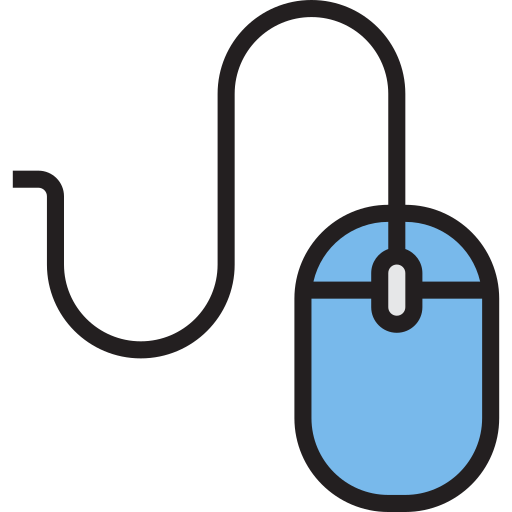
\includegraphics[width=1.4cm]{\icon{computerpack/017-mouse}}}
\newcommand{\imgkeyboard}{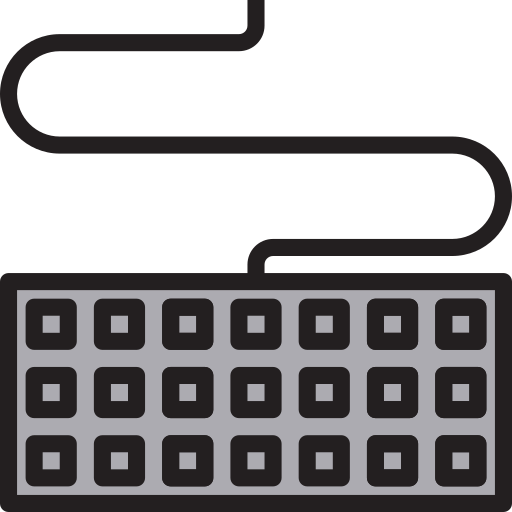
\includegraphics[width=1.4cm]{\icon{computerpack/024-keyboard}}}
\newcommand{\imgscreen}{\includegraphics[width=1.4cm]{\icon{computerpack/018-monitor}}}
\newcommand{\imglan}{
\includegraphics[width=1.4cm]{\icon{computerpack/023-lan}}}
\newcommand{\imglanred}{
\includegraphics[width=1.4cm]{\icon{computerpack/023-lan-red}}}
\newcommand{\imgcpu}{
\includegraphics[width=1.4cm]{\icon{computerpack/034-cpu}}}
\newcommand{\imgcpusmall}{
\includegraphics[width=1.0cm]{\icon{computerpack/034-cpu}}}

\newcommand{\imgdisplay}{\includegraphics[height=1.4cm]{\icon{computerpack/021-mobile}}}
\newcommand{\imgdisplaysmall}{\includegraphics[height=1.0cm]{\icon{computerpack/021-mobile}}}
\newcommand{\imgsim}{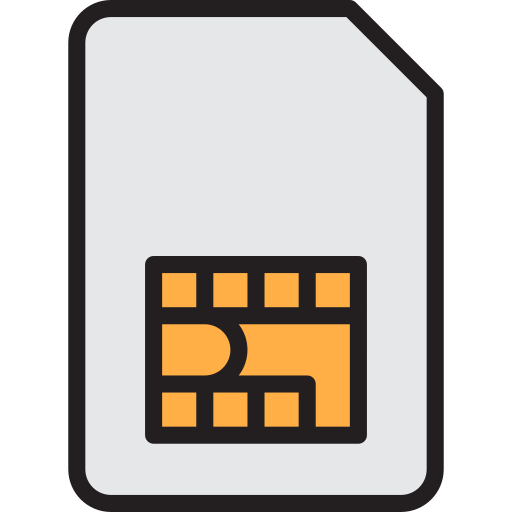
\includegraphics[height=1.4cm]{\icon{computerpack/008-sim-card}}}
\newcommand{\imgsimsmall}{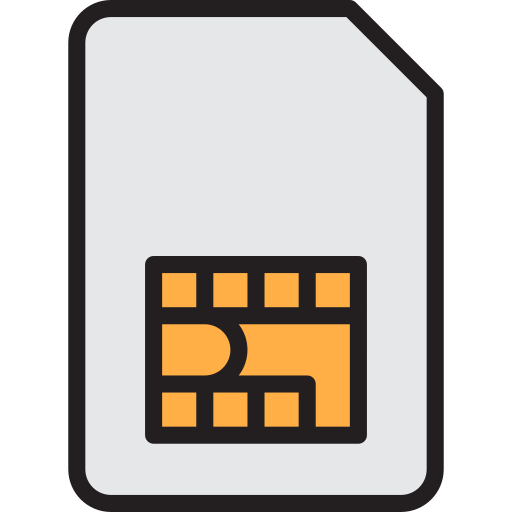
\includegraphics[height=1.0cm]{\icon{computerpack/008-sim-card}}}
\newcommand{\imgsd}{
\includegraphics[height=1.4cm]{\icon{computerpack/011-sd-card}}}
\newcommand{\imgsdsmall}{
\includegraphics[height=1.0cm]{\icon{computerpack/011-sd-card}}}
\newcommand{\imgcamera}{\includegraphics[width=1.4cm]{\icon{computerpack/035-camera}}}
\newcommand{\imgcamerasmall}{\includegraphics[width=1.0cm]{\icon{computerpack/035-camera}}}

\newcommand{\imgenclave}{\includegraphics[width=2.0cm]{\icon{enclave}}}
\newcommand{\imgenclavesmall}{\includegraphics[width=1.4cm]{\icon{enclave}}}
\newcommand{\imgenclavesmaller}{\includegraphics[width=1.0cm]{\icon{enclave}}}
\newcommand{\imgenenclavered}{\includegraphics[width=2.0cm]{\icon{sgx_red}}}
\newcommand{\imgenenclaveredsmall}{\includegraphics[width=1.0cm]{\icon{sgx_red}}}
\newcommand{\imguser}{
\includegraphics[height=2.0cm]{\icon{persons/user/user}}}
\newcommand{\imgusersmall}{
\includegraphics[height=1.4cm]{\icon{persons/user/user}}}
\newcommand{\imgattacker}{
\includegraphics[width=2.0cm]{\icon{persons/burglar}}}
\newcommand{\imgattackersmall}{
\includegraphics[height=1.4cm]{\icon{persons/burglar}}}
\newcommand{\imgcomputer}{
\includegraphics[width=2.0cm]{\icon{devices/client}}}

\newcommand{\imglock}{\includegraphics[width=0.3cm]{\icon{lock-icon}}}
\newcommand{\imglocklarge}{\includegraphics[width=0.5cm]{\icon{lock-icon}}}
\newcommand{\imgkeyyellow}{\includegraphics[width=0.5cm]{\icon{key-yellow}}}
\newcommand{\imgkeyred}{\includegraphics[width=0.5cm]{\icon{key-red}}}
\newcommand{\imgkeyblue}{\includegraphics[width=0.5cm]{\icon{key-blue}}}
\newcommand{\imgcertred}{\includegraphics[width=0.5cm]{\icon{certificate-red}}}
\newcommand{\imgcertyellow}{\includegraphics[width=0.5cm]{\icon{certificate-yellow}}}
\newcommand{\imgcertblue}{\includegraphics[width=0.5cm]{\icon{certificate-blue}}}

\newcommand{\imgdevil}{\includegraphics[width=0.6cm]{\icon{devil}}}

\let\oldding\ding% Store old \ding in \oldding
\renewcommand{\ding}[2][1]{\scalebox{#1}{\oldding{#2}}}% Scale \oldding via optional argument

\newcommand{\zero}{\ding[1.2]{171}\xspace}
\newcommand{\one}{\ding[1.2]{172}\xspace}
\newcommand{\two}{\ding[1.2]{173}\xspace}
\newcommand{\three}{\ding[1.2]{174}\xspace}
\newcommand{\four}{\ding[1.2]{175}\xspace}
\newcommand{\five}{\ding[1.2]{176}\xspace}
\newcommand{\six}{\ding[1.2]{177}\xspace}
\newcommand{\seven}{\ding[1.2]{178}\xspace}
\newcommand{\eight}{\ding[1.2]{179}\xspace}
\newcommand{\nine}{\ding[1.2]{180}\xspace}
\newcommand{\ten}{\ding[1.2]{181}\xspace}

\newcommand{\risc}{RISC-V\xspace}
\newcommand{\ce}{controller enclave\xspace}
\newcommand{\ces}{controller enclave\xspace}
\newcommand{\Ce}{Controller enclave\xspace}
\newcommand{\Ces}{Controller enclave\xspace}
\newcommand{\app}{application enclave\xspace}
\newcommand{\App}{Application enclave\xspace}
\newcommand{\apps}{application enclaves\xspace}
\newcommand{\Apps}{Application enclaves\xspace}


\newcommand*\circled[1]{\tikz[baseline= (char.base)]{
            \node[shape=circle,draw,inner sep=0.3pt] (char) {\(#1\)};}}

\newcommand{\blue}[1]{\textcolor{black}{#1}}
\newcommand{\red}[1]{\textcolor{red}{#1}}


\newcommand{\figsaver}[0]{\vspace{-5pt}}
\newcommand{\parasaver}[0]{\vspace{-2pt}}

\newif\ifremoveall{}
\removealltrue{}

\ifremoveall{}
\newcommand{\aritra}[1]{\textbf{\emph{ #1 \colorbox{green}{[Aritra]}}}}
\newcommand{\ip}[1]{\textbf{\emph{ #1 \colorbox{cyan}{[Ivan]}}}}
\newcommand{\moritz}[1]{\textbf{\emph{ #1 \colorbox{yellow}{[Moritz]}}}}
\newcommand{\srdjan}[1]{\textbf{\emph{ #1 \colorbox{blue}{[Srdjan]}}}}
\newcommand{\todo}[1]{\textcolor{red}{TODO: \@#1}}
\newcommand{\todoref}{\textcolor{red}{[ref]}}
\newcommand{\citneed}{[\textcolor{red}{cit}] }
\else
\newcommand{\aritra}[1]{}
\newcommand{\ip}[1]{}
\newcommand{\moritz}[1]{}
\newcommand{\todo}[1]{}
\newcommand{\todoref}[1]{}
\newcommand{\citneed}[1]{}
\fi


\newcommand{\name}{\textsc{PIE}\xspace}
\newcommand{\tool}{\textsc{\name{} API}\xspace}
\newcommand{\device}{\textsc{Device}\xspace}

\newcommand{\usb}{\texttt{USB}\xspace}
\newcommand{\tls}{\texttt{TLS}\xspace}

\def\nameenclave{platform-wide enclave\xspace}
\def\Nameenclave{Platform-wide enclave\xspace}

\newcommand{\sphw}[0]{specialized hardware\xspace}
\newcommand{\Sphw}[0]{Specialized hardware\xspace}


%%%%%%%%%%%%%%%%%%%%%%
%savetrees
\usepackage[
all=normal,floats=tight
,paragraphs=tight
% ,wordspacing=tight
,mathspacing=tight
% ,mathdisplays=tight
]{savetrees}
%%%%%%%%%%%%%%%%%%%%%%

% \newcommand{\myparagraph}[1]{\par\emph{#1.}\xspace}
\newcommand{\myparagraph}[1]{\paragraph{#1}}

\newcounter{para}
% \newcommand{\mypara}[1]{\refstepcounter{para}\emph{\thepara}.\space\emph{#1}.\xspace}
\newcommand{\mypara}[1]{\refstepcounter{para}\paragraph{\thepara.\space{}#1}}
% \newcommand{\mypara}[1]{\paragraph{#1}}
%\newcommand\mypara{\par\refstepcounter{para}\thepara\space}

%------------------------------------------------------------------------------
%                                Space savers.
%------------------------------------------------------------------------------
% This mylist environment indents items, and saves less space than the above.
\newcounter{myctr}
\newenvironment{mylist}{\begin{list}{\arabic{myctr}.}
{\usecounter{myctr}
\setlength{\topsep}{1mm}\setlength{\itemsep}{0.5mm}
\setlength{\parsep}{0.5mm}
\setlength{\itemindent}{1mm}\setlength{\partopsep}{0mm}
\setlength{\labelwidth}{-2mm}
\setlength{\leftmargin}{0mm}}}{\end{list}}

\newenvironment{mylist_indent}{\begin{list}{\arabic{myctr}.}
{\usecounter{myctr}
\setlength{\topsep}{1mm}\setlength{\itemsep}{0.5mm}
\setlength{\parsep}{0.5mm}
\setlength{\itemindent}{1.5mm}\setlength{\partopsep}{1mm}
\setlength{\labelwidth}{-2mm}
\setlength{\leftmargin}{1mm}}}{\end{list}}

% Space saving List environment for itemizing.
\newenvironment{mybullet}{\begin{list}{\bullet}
{\setlength{\topsep}{1mm}\setlength{\itemsep}{0.5mm}
\setlength{\parsep}{0.5mm}
\setlength{\itemindent}{0mm}\setlength{\partopsep}{0mm}
\setlength{\labelwidth}{-2mm}
\setlength{\leftmargin}{0mm}}}{\end{list}}


% Break characters in the reference
\expandafter\def\expandafter\UrlBreaks\expandafter{\UrlBreaks
  \do\a\do\b\do\c\do\d\do\e\do\f\do\g\do\h\do\i\do\j
  \do\k\do\l\do\m\do\n\do\o\do\p\do\q\do\r\do\s\do\t
  \do\u\do\v\do\w\do\x\do\y\do\z\do\A\do\B\do\C\do\D
  \do\E\do\F\do\G\do\H\do\I\do\J\do\K\do\L\do\M\do\N
  \do\O\do\P\do\Q\do\R\do\S\do\T\do\U\do\V\do\W\do\X
  \do\Y\do\Z}
  
  

\graphicspath{{images/}}

\begin{document}
%\title{\name: Platform Execution Environment \\ Enclave to Exclave} 
\title{\name: A Platform-wide TEE} 

\iffalse
\author{
    \IEEEauthorblockN{Moritz Schneider\textsuperscript{*}, Aritra Dhar\textsuperscript{*}, Ivan Puddu, Kari Kostiainen, Srdjan \v{C}apkun}
    \IEEEauthorblockA{Department of Computer Science\\
    ETH Zurich}
}
\fi

\iffalse
\begingroup\renewcommand\thefootnote{*}
\footnotetext{Equal contribution}
\endgroup
\fi

%\acmConference[Submission]{}{}

\begin{abstract}


% \ad{Draft 1: Flow = traditionally CPU is the central part -- specialized hardware can do operations more efficiently than CPU e.g., GPU -- TEEs are great for CPU -- not so great for peripherals -- adding peripherals to the TEE can blow up the TCB size -- we need configurable TCB that enforce least privilege -- platform-wide enclaves -- provides platform-wide attestation -- ensures the integrity of the state of the platform -- prototype -- number}
%Traditionally, the CPU is considered to be the primary execution unit of a computing platform. However, \sphw (such as a GPU) outperforms CPUs for specialized workloads by orders of magnitude. %Some other applications heavily depend on peripherals for their data source/sink (e.g., IO devices, sensors).
%These advancements in \sphw shift the CPU's traditional role from the primary execution unit to a mere coordinator of \sphw.
%Nevertheless, the security of such systems is not widely investigated and more focused on the traditional CPU-centric model by employing trusted execution environments (TEEs). %For most existing TEEs, the protection mechanisms only apply to the applications on the CPU by isolating them from the attacker-controlled OS, leaving \sphw devices unprotected.
% Often, these external devices handle sensitive data, hence, the applications' correct operations rely on their integrity and authenticity. Protecting such applications running on the CPU cores can be achieved by leveraging existing mechanisms such as Trusted execution environments (TEE). However, for most of the existing TEEs, the protection is only applied to the applications on the CPU cores by isolating them from the attacker-controlled OS, leaving external hardware devices unprotected. Integration with TEEs and external devices is possible in specific platforms, but with the cost of increasing the TCB massively.

While modern computing architectures rely on \sphw such as accelerators to provide performance and functionality, trusted execution environments (TEEs), one of the most promising recent developments in security, can only protect code confined in the CPU, limiting TEEs potential and applicability to a handful of applications. 
We observe that the TEEs' hardware trusted computing base (TCB) is fixed at design time, forcing users to rely on (mostly untrustworthy) software to allow peripherals into the TEE. Based on this observation, we propose \name, a secure platform design with a configurable hardware and software TCB, which allows us to support \sphw while ensuring the least privilege principle.
We introduce two new security properties relevant to such systems: \emph{platform-wide attestation} and \emph{platform awareness}. Platform-wide attestation allows to remotely verify the platform's current state, including the state of \sphw devices and how they are connected with each other, whereas platform awareness defines how the enclave reacts upon a change in connected devices. Together, these allow to attest to the hardware configuration of a system and check that only the trusted hardware with the right version of its firmware is part of the TCB (platform-wide attestation) and will stay part of the TCB for the whole execution (platform awareness). %, as \name makes its enclaves aware of any peripheral and configuration change.
Finally, we present a prototype of \name based on RISC-V's Keystone to show that such systems are feasible with only around 600 lines added to the software TCB, without compromising performance.


\end{abstract}
\maketitle
%\thispagestyle{empty}

\section{Introduction}
\label{integriscreen:sec:intro}

In the previous chapter (Chapter \ref{ch:integrikey}) we describe \integrikey that provides second factor for the integrity of the user input coming from keyboard. However, this integrity guarantee is purely limited the keyboard input and does not take account of what the user is seeing on the screen. In other wards, \integrikey is oblivious to the the user's \emph{intent}. We use the term intent to establish the connection between what the user is seeing on the display and what the user is typing in response to that. Similar, to \integrikey, we assume an attacker that control the software stack including the OS and hypervisor of the host that the user has. A large class of web-based services and applications (e.g., online banking or remote database access) uses modern user interfaces (UIs) displayed on the browser to interact with the user. In all of these UIs, the user's intended input is displayed on the host's screen. Despite what a compromised host might attempt to do in the background, users communicate their intention by entering and modifying the values shown on the screen until they are satisfied with what they see or abort if they are prevented from doing so.

Existing literature looked into this general idea of supervising user input on an untrusted host to extract user intention. However, these works relied on the assumption that the host is only partially compromised by assuming the existence of either a trusted virtual machine~\cite{gyrus}, an operating system~\cite{binder}, or an \emph{attester} application~\cite{nab} that captures the user's input and relays them to the server. 

Motivated by the increase in computer vision capabilities of various camera-enabled devices (e.g., augmented reality headsets~\cite{TimCookAR, HoloLens2}, smart home camera assistants~\cite{fleck2008smart, lenovoSmartHome} and smartphones~\cite{wald2018real, smartphonesCV}), we propose a new concept that we call \emph{visual supervision of user's intent}. This concept works by leveraging a camera-equipped device (such as a smartphone) to capture the host's screen when the user provides input to the web UIs. A trusted application on the smartphone then extracts these user inputs and sends them to the remote server using its own communication channel. Upon receiving these data from the smartphone, the remote server compares them with the input data in the response packets received from the host. Thus, the attacker-controlled host is prevented from either generating arbitrary user input or from modifying the input provided by the user.


In summary, this chapter makes the following main contributions:

\begin{enumerate}
  
	\item \textbf{System design.}
	We propose and describe \sysname, a system that protects the integrity of the user's input to a remote server by using a device equipped with a camera to visually supervise the user's interaction with an untrusted host thus preventing various advanced UI attacks that the adversary might attempt.


	\item \textbf{Prototype \& experimental evaluation.}
	To evaluate the feasibility of the approach on recent smartphones, we build a fully functional prototype of the \sysname system and test it with three different devices against a range of automated attacks.

\end{enumerate}

\section{Background}
\label{sec:background}

\paragraph*{Keystone}
Keystone~\cite{keystone} is a TEE framework based on RISC-V that utilizes physical memory protection or PMP to provide isolation. PMP is part of the RISC-V privilege standard~\cite{riscv2019privspec} and it allows to specify access policies that can individually allow or deny reading, writing, and executing for a certain memory range. E.g., PMP can be used to restrict the operating system (OS) from accessing the memory of the bootloader. Every access request to a prohibited range gets trapped precisely in the core and results in a hardware exception. Keystone relies on a low-level firmware with the highest privilege, called security monitor (SM), to manage the PMP. 

The SM maintains its own memory separate from the OS and protected by a PMP entry. It also facilitates all enclave calls, e.g., it creates, runs, and destroys enclaves. The SM configures the PMP so that the OS can no longer access the enclave's private memory. Upon a context switch, the SM re-configures the PMP to allow or block access to the enclave. E.g., during a context switch from an enclave to the OS, the SM changes the PMP configuration such that access to the enclave memory is prohibited. Conversely, on a context switch back to the enclave, the PMP gets reconfigured to allow accesses to enclave memory. 
Because the SM is critical for the security of any enclave and the whole system, it aims to be very minimal and lean. As such, the SM is orders of magnitudes smaller than hypervisors and operating systems (15k LoC vs millions LoC~\cite{torvalds2020linux,barham2003xen}). There are also efforts to create formal proofs for such a SM~\cite{lebedev2019sanctorum}. Keystone also provides extensions for cache side-channel protections using page coloring or dynamic enclave memory. 

\paragraph*{Device Tree}
The device tree is a list that accurately describes the physical memory mappings of a platform. It describes the central processor, i.e., its speed, its ISA, and at what address its cache starts. It also includes the DRAM base address and various other components on the die, such as various internal and external buses. It is usually used by the bootloader and the OS to bootstrap the system. As some peripherals cannot be detected automatically, they must be present in the device tree, as otherwise they will not get recognized by the OS. The device tree is usually burnt into ROM and available to the bootloader and the OS. It can therefore be considered trusted.

% \subsection{Hardware Background}
% \subsubsection{RISC-V}
% RISC-V is a modern open-source instruction set architecture (ISA). In recent years, RISC-V has sparked immense interest by industry and academia, with many software and hardware proposals. As a consequence, multiple open source cores that implement various subsets of the RISC-V standard have emerged~\cite{ariane,asanovic2016rocket,riscy,asanovic2015boom}. Software-wise, RISC-V is supported by many projects, e.g., by GCC, linux, and QEMU amongst others. RISC-V has also become a popular prototype platform for security research~\cite{weiser2019timber,costan2016sanctum,keystone}.

% \subsubsection{Physical Memory Protection}
% Physical memory protection (PMP) is part of the RISC-V privilege standard~\cite{riscv2019privspec}. It allows to specify access policies based on a physical memory range. The access policies can individually allow or deny reading, writing, and executing for a certain memory range. For example, PMP can be used to restrict the operating system (OS) from accessing the memory of the bootloader. Every access request into a prohibited range gets trapped precisely in the core and results in a hardware exception. There are a fixed number of available PMP entries, typically 8 or 16~\cite{riscv2019privspec}, each of which allows to specify a separate memory range. Since PMP is part of the standard, it is already included in many currently available cores~\cite{riscy,asanovic2016rocket}.



% \subsection{Trusted Execution Environments (TEE)}

% Traditional trusted execution environments (TEE) introduce a small protected program called enclave. An enclave runs on the processor isolated from the attacker-controlled OS and hypervisor. Enclaves provide code integrity and data confidentiality, even in the presence of a physical adversary. Integrity of the enclave code at the time of deployment is ensured by remote attestation while the enclave data confidentiality and integrity during runtime are provided by various hardware mechanisms. For example, Intel SGX uses memory encryption and the Memory Management Unit (MMU).
%, whereas RISC-V Keystone~\cite{keystone} uses PMP to isolate the enclave data from the untrusted OS and other applications. 

%\subsection{Keystone}


\section{Problem Statement}
\label{sec:problemStatement}

% \begin{figure}[t]
%     \centering
%     \includegraphics[width=0.9\linewidth]{images/cpu_bus_peripheral-Page-1.pdf}
%     \caption{A typical bus architecture of a platform where the cores are connected to on-chip bus controllers such as PCI and USB, wich are in turn connected to external \sphw devices. E.g, the GPU and the keyboard is connected via the PCI-E controller and SPI bus respectively.}
%     \label{fig:bus}
% \end{figure}


Modern platforms are composed of complex heterogeneous \sphw, from simple sensors that measure temperature or humidity to complex accelerators for machine learning. All these components are connected to the CPU over buses (e.g., PCI, USB, etc.). % as depicted in Figure~\ref{fig:bus}.
Many modern applications are critically dependent on such \sphw, and often they handle sensitive data, e.g., patient records for machine learning. Thus, these \sphw{}s' authenticity and integrity are critical, and the data they handle must remain confidential. 
% We list three such applications in the following:

% \paragraph{Application 1: Isolated execution on accelerators} 
% Many science fields require a vast amount of computation power, which a general-purpose processor can no longer provide. In recent times, specialized hardware which is very efficient for one specific problem is used in the form of accelerators, e.g., machine learning accelerators in the cloud. Such applications often handle sensitive data such as patient records and require isolation from the OS and other applications running on the same GPU. %Besides, these accelerators might need to be connected to live measurements such as a camera and process the inputs in real-time.

% \paragraph{Application 2: Trusted sensor readings}
% Safety-critical industrial and medical devices rely on measurements of critical sensors. E.g., a pressure sensor provides data to the industrial controller, who decides when to open a safety valve.
    
% \paragraph{Application 3: Trusted path for IO devices} A user uses her IO devices (keyboard, mouse, display, etc.) to interact with an online banking application running on her device. The user wants to verify that the banking application is exclusively accessing her IO devices. In this case, the user wants to harden her system against a potentially compromised software stack.

%\moritz{Should we go more into the direction of remote systems vs hardening measures?}

Applications that handle sensitive data and use a \sphw device can be deployed securely with one of the following three existing approaches: 1) designing a fully dedicated system, or 2) renting a dedicated virtual machine and placing trust in the hypervisor, or 3) relying on the OS. None of these approaches to be satisfactory due to lack of generality, cost, and the need to trust codebases with millions of lines of code~\cite{torvalds2020linux,barham2003xen}. Existing TEEs such as Intel SGX, RISC-V Keystone, ARM TrustZone, etc., provide security guarantees only to the applications running on the CPU cores leaving \sphw unprotected. Moreover, SGX and Keystone enclaves rely on the untrusted OS to communicate with \sphw. On the other hand, ARM TrustZone provides isolated communication between the enclaves and components such as a touchscreen, fingerprint sensor, but requires trusting the entire secure OS, including device drivers not used by the enclave.  %Graviton~\cite{volos2018graviton} proposes isolated enclaves on the GPU that communicate securely with the SGX enclaves. But its geared to a GPU can cannot be extended to generic \sphw.


\subsection{Attacker Model}
\label{sec:problemStatement:attackerModel}

The attacker model is tightly coupled with the type of \sphw. We separate the \sphw into two main classes due to their distinct effect on the attacker model: 
%\sphw that explicitly interact with their physical environment and those that do not. Intuitively, sensors interact with their environment by taking measurements. Accelerators, however, do not explicitly interact with the real-world. The \sphw classes and their respective attacker models are described in the following:

\begin{enumerate}
\item \emph{\Sphw with physical interaction:}
\Sphw that interact with their environment range from input-only, such as input peripherals (e.g., mouse, keyboard) and sensors (e.g., temperature sensor) to output-only devices (e.g., monitor) and combined IO devices (e.g., touchscreen). For any such device, a local physical adversary can manipulate the environment and thus the input (and potentially the output). E.g., a physical adversary can point a laser at a light sensor, thus changing the sensor's reading but not the room's overall light intensity. Hence, any \sphw that interacts with its physical environment cannot tolerate a physical adversary.

\item \emph{\Sphw without physical interaction:}
There are \sphw units that do not explicitly interact with their environment. They draw power and produce heat, but their input and output are not related to the environment. GPUs and other accelerators are the prime examples of this class of \sphw, for whom a local physical adversary can be tolerated. 
\end{enumerate}

In this paper, we assume a remote attacker that remotely controls the entire software stack, including the OS and hypervisor. While the remote attacker model is a weaker assumption compared to the local physical one considered in the existing TEEs, the former covers a wide class of \sphw (e.g., \sphw with physical interaction) that cannot tolerate physical attackers. Hence, the attacker cannot access the platform of the \sphw physically or hot-swap a device. Note that the untrusted OS is still in charge of managing \sphw devices, and thus is able to remap the devices or send a reset or power-off signal.
We assume that the CPU firmware is trusted. Similar to existing TEE proposals, side channel attacks remain out of scope~\cite{costan2016intel} in our adversary model. However, we will discuss the implications of our proposal on existing side channel attacks and defenses in \Cref{sec:securityAnalysis}. Finally, we consider denial-of-service attacks to be out of scope in this paper. 


\subsection{Challenges}
\label{sec:problemStatement:challenges}
%\moritz{Needs to be adapted to intro. (and better formulated).}
As mentioned above, several approaches could be pursued to integrate \sphw into a TEE. Among them, we investigate approaches that reuse components of existing systems as much as possible, both in terms of software and in terms of hardware.  
%A modern platform's computation capability is distributed over \sphw units with the CPU acting as a coordinator. For computation tasks on sensitive data, the data's integrity and confidentiality is crucial in all devices. The TCB should remain configurable and only include the application running on the CPU and the driver and the firmware of the \sphw device it is accessing. 
%In this paper, we address this by investigating enclaves that span an entire platform, which we call \emph{\nameenclave{}s}. In addition, the hardware and software TCB of a \nameenclave{} should be configurable and thus adhere to the principle of least privilege. 
%In this paper, we investigate enclaves that span an entire platform as distributed enclaves constructed from individual and asynchronous enclaves.
This approach leaves the OS in a supervisor role, liaising between the isolated environments and \sphw, similar to memory in traditional TEEs (c.f. Section~\ref{sec:background}). But, this decision leaves leeway for privileged adversaries to break the system's isolation. We therefore need to consider both existing threats to traditional TEEs and emerging threats due to the nature of a reconfigurable hardware TCB. 
% As analyzed in CPU-centric TEEs~\cite{checkoway2013iago}, this approach leaves leeway for privileged attackers to break the system's isolation. We therefore need to take into account both these threats and the ones that emerge due to the nature of a reconfigurable hardware TCB. 
We analyze these in more detail in the next three paragraphs.

% Extending the TEEs to the entire platform is non-trivial and comes with several challenges, especially in the application scenarios that we discussed previously in Section~\ref{sec:problemStatement}. There exists a few proposals of TEEs that consider \sphw, such as solutions~\cite{VButton,SeCloak} based on ARM TrustZone. However, they require all the \sphw present in the platform in the TCB. We consider a \name to be a combination of multiple TEEs on individual components, e.g., a TEE on the CPU~\cite{sgx,keystone} and one on the GPU~\cite{volos2018graviton}. A \name{} should provide similar guarantees as traditional TEEs and eventually pave the way for secure computation on an entire platform.

\myparagraph{Secure communication}
Traditionally, the OS or the hypervisor act as the bridge between applications and \sphw. They are responsible to set-up these communication links properly, and can not only observe the data exchanged between different components, but also tamper with it.
%However, OS and hypervisors are usually large codebases with hundreds of lingering vulnerabilities~\cite{checkoway2013iago,suzaki2011memory}
As they are not trusted in our attacker model, we need to ensure that each components establishes a secure link with each other. This is not trivial, as the OS is untrusted and may not cooperate. % of the OS is required to avoid bloating the enclaves' TCB.
% Hence, secure communication between the enclave on the CPU and the \sphw provides isolation from all other components on the platform. 
Finally, the fact that several accelerators may need to support a form of multi-tenant isolation (e.g., multiple tasks on a GPU), requires careful consideration, as sensitive data within a isolated environment in \name should remain confidential irrespective of what else is running on the system.

% \Sphw such as a GPUs also require some form of multi-tenant isolation to be able to execute multiple concurrent separated sensitive calculations. Hence, no enclaves can observe such communications between the other enclaves on the processor and \sphw.


\myparagraph{Remote Attestation}
Remote attestation is a key part of any TEE. However, with multiple \sphw devices and enclaves on the CPU making up a distributed enclave, the straight-forward approach to just individually attest to every component is vulnerable to time-of-check-time-of-use attacks. Several attestations (one for each component of the TEE) must be linked with a guarantee that nothing has changed in the components already attested since the last attestation. Without this guarantee, an attacker could tamper with the configuration of already attested enclaves and thus tricking the remote verifier.

% Therefore, the remote attestation must either happen atomically or consider changes in between attestations, and it needs to cover the enclave on the processor itself, the relevant \sphw, and their communication configuration.

% a remote verifier must obtain a signed attestation report about an enclave of \name{}. E.g., a user wants to remotely attest that the \nameenclave{} in the cloud contains a specific accelerator. The user also wants to attest the communication link is isolated from other applications and the legacy software stack (see secure communication). Existing systems are statically designed and cannot dynamically include \sphw in the TCB. E.g., in Intel SGX, users are forced to trust the Intel ME even if it is not used. The remote verifier does not want to trust all \sphw connected to the platform, but only the relevant devices for the target enclave, e.g., the GPU for the ML workload. 

\myparagraph{Runtime attacks}
Remapping attacks are also relevant during runtime, as the OS still manages the memory. Well-timed disconnects or memory remappings could result in leakage of confidential data, e.g., if an adversary remaps a \sphw device and replaces it with a malicious device, the CPU enclave should not share sensitive data with the new device. 

% When including the \sphw into enclaves, changes in the platform's components has to be considered. E.g., a GPU that is handing sensitive data could be swapped with a different GPU during runtime. In such a scenario, the enclave should stop sending sensitive data to the GPU until it re-attest the new GPU. Hence, the enclave has to react to the external events i.e., it has to be aware of the platform's state. The full state of a system is too detailed to be processed every time it changes or to meaningfully assess whether it is safe for a remote stakeholder to provide its data. Therefore, this last challenge requires concretely defining what parts of the state (and state transitions) of a system are relevant for the security of \name{}.

%%% This has been removed cause it is now at the beginning
% \myparagraph{Compatibility with existing Ecosystem} 
% In addition to all of the above challenges, changes to existing applications, drivers, and \sphw firmware should be kept as small as possible. Note that the attestation of the \sphw may require some hardware modification in the existing \sphw (e.g., adding key storage, crypto co-processor etc.). 


\section{Overview of Our Approach}
\label{sec:overview}


In this section, we provide an overview of our approach \name and introduce \emph{\nameenclave{}s}. \Nameenclave{}s dynamically extend the TCB of traditional TEEs running on the CPU to the \sphw. \Nameenclave{}s consist of multiple distributed enclaves that run on various hardware components such as the CPU and \sphw as shown in Figure~\ref{fig:new_system}. \Nameenclave{}s aim to provide similar security properties as traditional enclaves, such as integrity, attestation, and data isolation from other enclaves and the attacker-controlled OS. 

\begin{figure}[t]
    \centering
	\includegraphics[trim={0 8cm 15cm 0}, clip, width=\linewidth]{chapters/PIE/images/pwe_idea.pdf}
    \caption[\Nameenclave{}s consists of different applications and \sphw]{Two \nameenclave{}s are highlighted by blue and yellow outlines. The blue one consists of \texttt{Encl1}, a keyboard that is connected over the memory-mapped SPI bus and a GPU connected over PCI through DMA. This case represents a trusted path scenario where user requires both input and output. The second consists of \texttt{Encl2} and a GPU connected over PCI through DMA. The second one represents a usecase such as executing machine learning workload in the GPU cores.}
    \label{fig:new_system}
\end{figure}



\subsection{Enclaves within a \nameenclave}
\label{sec:overview:enclaves}

A \nameenclave{} consists of multiple enclaves that run on different hardware components and securely communicate with each other. A \nameenclave{} typically contains several interconnected processor-local enclaves and \sphw enclaves. In the following, we describe the two main enclave types that form a \nameenclave{}.

\myparagraph{Processor-local enclaves}
\label{sec:overview:enclaves:processorEnclave}

Processor-local enclaves are equivalent to traditional enclaves and their runtime memory must be isolated from the OS and should only be accessible to the enclave itself. To achieve that, we use physical memory protection (PMP) from the RISC-V privilege standard~\cite{riscv2019privspec} as introduced by Keystone.

We further differentiate two types of processor-local enclaves: \app{}s, and \ce{}s which encapsulate the application-specific, and driver logic, respectively. As seen in Figure~\ref{fig:sharedMemory}, $AE_1$, and $CE_1$ are the \app, and \ce in the blue-outlined \nameenclave of Figure~\ref{fig:new_system}. The \ce also provides isolation between the \apps in a scenario where multiple \apps want to access a certain \sphw. Therefore, \ce enforces access control on the connected \apps in terms of how a certain \sphw can be accessed, e.g., exclusive access to a keyboard or shared concurrent access to a GPU. 
% $AE_1$ uses $CE_1$ to communicate with $P_1$ that is a \sphw enclave which we discuss in the following. 

\myparagraph{Enclaves on \sphw}
\label{sec:overview:enclaves:peripheralEnclave}
Most \sphw run some firmware or even some custom code (e.g., graphic shaders) which has to be included in the TCB of a \nameenclave.
E.g., the GPU and its firmware in Figure~\ref{fig:new_system} is part of the yellow \nameenclave. Since a remote verifier also wants to attest to the \sphw, they have to be modified to support attestation. However, we stress that these modifications  remain rather small (refer to~\Cref{sec:eval:impl:usecase}) and usually only involve small changes in the device firmware. %Essentially, one only has to add a certificate from the manufacturer for a secret key stored in the \sphw.

\begin{figure}[tbp]
     \centering
     %\includestandalone[width=0.9\linewidth]{images/tikz/approach}
     %\includegraphics[trim={0 15cm 28cm 0}, clip, width=0.5\linewidth]{approach.pdf}
    %  \includegraphics[trim={0 12cm 27cm 0}, clip, width=0.5\linewidth]{approach_combined.pdf}
     \includegraphics[width=0.4\linewidth]{chapters/PIE/images/softwaredesign.pdf}
     
     %\caption{Example configuration where a red CPU enclave shares some memory with a blue CPU enclave and another shared buffer with a GPU. The solid color memory cells correspond to the private enclave memory regions, and the cells with mixed color denote shared memory regions.}
     \caption[Three example \nameenclave{}s in \name{}'s software design]{Three example \nameenclave{}s in \name{}'s software design with \app{}s (AE), \ce{}s (CE), a GPU, and a keyboard. Note that the red \nameenclave{} is spanning over two external devices and \ce{}s isolate the data from the different \app{}s.}
     \label{fig:sharedMemory}
\end{figure}

\subsection{Communication with \sphw}
\label{sec:approach:comm}

First, we need to understand how devices are managed by platform using a structure called \emph{device tree}.

\myparagraph{Device Tree}
The device tree is a list that accurately describes the physical memory mappings of a platform. It describes the central processor, i.e., its speed, its ISA, and at what address its cache starts. It also includes the DRAM base address and various other components on the die, such as various internal and external buses. It is usually used by the bootloader and the OS to bootstrap the system. As some peripherals cannot be detected automatically, they must be present in the device tree, as otherwise they will not get recognized by the OS. The device tree is usually burnt into ROM and available to the bootloader and the OS. It can therefore be considered trusted.

\myparagraph{Secure communication}
To enable processor-local enclaves and \sphw enclaves to securely communicate, we make the observation that these devices generally communicate over mapped address regions: They either use an address range that is not reflected in DRAM, so-called memory-mapped-input-output registers (MMIO), or a shared DRAM region accessed via direct memory access (DMA). To maximize compatibility with existing drivers and \sphw, we chose not to change this behavior. Instead, we isolate the address regions that are used in this communication. Existing hardware mechanisms like PMP already allow restricting access to a specific address region. Until now, such hardware mechanisms have been predominantly used to restrict memory access, but in our design, they also allow to restrict access to other address regions that are not in the DRAM range\footnote{E.g., DRAM could occupy the address range \texttt{0x8000000 - 0xF0000000}, whereas other \sphw such as UART could reside at \texttt{0x4000000 - 0x4001000}.}. Note that these address regions from \sphw are either i) static, i.e., hardcoded and provided to the SM in the form of a trusted device tree file, or ii) dynamic, i.e., configured at runtime by the SM. In our design, the SM always maintains a complete overview of all such regions and only allows a single enclave to access an address region of a \sphw.

While we made the changes mentioned above to the SM to support \sphw with both MMIO and DMA, they also enable a new way for enclaves to communicate: shared memory. This reflects a major difference to traditional TEEs because until now; most traditional enclaves could only communicate through the untrusted OS\footnote{Concurrent work~\cite{yu2020elasticlave} has also shown how shared memory can improve the performance of enclaves significantly.}. 
% By supporting DMA regions for \sphw, our design also implicitly supports shared memory between enclaves. 
%Figure~\ref{fig:sharedMemory} shows an example shared memory configuration of our design.


\subsection{Changes within a \nameenclave{}}
\label{sec:overview:awareness}

The untrusted OS manages \sphw devices; hence the OS could remap any device or send a reset signal. E.g., a GPU that is handing sensitive data could be shut down by the OS and remapped to a different GPU during runtime. In such a scenario, the enclave should stop sending sensitive data to the GPU until the remote verifier re-attests the new GPU. Hence, the enclave has to react to these external events, i.e., it has to be aware of the platform's state. 
In traditional TEEs, enclaves are self-sufficient isolated entities and are only dependent on themselves. 
Therefore, they can only be in two states: running or stopped. \Nameenclave{}s are more complex since they can contain multiple enclaves, all of which could be running, stopped, or even killed. \Nameenclave{}s have to react correctly upon any of these events to keep the data confidential. We achieve this by expanding the enclave lifecycle and adding two new events: connect and disconnect. The asynchronous nature of these events requires a detailed analysis of the security of the entire system, e.g., a well-timed disconnect could lead to data leaks across shared memory regions. We solve this issue by assigning ownership of the shared memory among the enclaves that are accessing that memory. Upon any external events, if one of the participating enclaves dies, the sole ownership is transferred to the remaining one (more details in \Cref{sec:lifeycle}). Therefore, the components in the \nameenclave are \emph{platform-aware} since they are aware of any change within their ecosystem.


\subsection{Attestation of a \nameenclave{}}

Since a \nameenclave{} consists of multiple distributed enclaves, attestation poses another challenge. Individual attestations to each enclave that make up a \nameenclave{} could be vulnerable to timely manipulations by an attacker to cause time-of-check-to-time-of-use (TOCTOU) issues. To provide a platform-wide attestation, we need to chain attestation reports of all the components of a \nameenclave. This includes the attestation report of the enclaves and \sphw firmware. Attestation of the \sphw firmware is achieved by signing a challenge message with the key embedded in the \sphw (refer to Section~\ref{sec:overview:enclaves:peripheralEnclave}).
The attestation of a \nameenclave{} could either be a one-time attestation that results in a huge chain of reports or individual attestations of all entities that can be combined by the verifier. 
We show that individual attestations provide more flexibility for the verifier and are secure against TOCTOU attacks by adding unique identifiers to enclaves and appending all connected enclaves' IDs to the attestation report.
%% Ivan: I have removed the following cause it adds no value to the discussion at this point 
%Surprisingly, this even remains true when identifiers are reused. 


% The full state of a system is too detailed to be processed every time it changes or to meaningfully assess whether it is safe for a remote stakeholder to provide its data. Therefore, this last challenge requires concretely defining what parts of the state (and state transitions) of a system are relevant for the security of \name{}.

\begin{figure}[tbp]
    \centering
    \includegraphics[width=0.7\linewidth]{chapters/PIE/images/cpu_bus_peripheral-Page-5.pdf}
    \caption[Interactions between \nameenclave's components]{An example scenario that illustrates interaction between \nameenclave components.}
    \label{fig:overviewtime}
    % \vspace{-1em}
\end{figure}

\subsection{Summary of Interactions}
To summarize all interactions between the components of a \nameenclave, we present an example scenario in Figure~\ref{fig:overviewtime} with an \app{}, a \ce{}, and a \sphw device. The scenario is as the following:
\begin{enumerate}
    \item[\one] The OS creates and configures the \ce{} and hands over control to the SM. The SM then revokes the OS's access permissions to the private memory regions of the \ce{}.
    \item[\two] The OS requests SM to connect \ce{} with the \sphw device. The SM sets up a new shared memory region and enables access only to the \ce{}.
    \item[\three] Similar to the \ce, the OS creates and configures the \app{}, and then, once again, the SM revokes access to the private memory of the enclave.
    \item[\four] The OS calls the SM to establish a shared memory region between the \ce and the \app. 
    \item[\five] After a remote verifier attests to all enclaves (using the \app as the entry point), sensitive data can be transmitted, and the normal operation starts.
    \item[\six] Any disruption, i.e., a disconnection of the \sphw device, leads to an asynchronous disconnect, where the sole ownership of the shared memory between the device and the \ce{} moves to \ce(see Section~\ref{sec:lifeycle}). Moreover, the enclaves may halt execution until re-attested.
\end{enumerate}

% \subsection{Software Design}

% The last major challenge is to make \name easy to adapt for existing software and \sphw (refer to challenge \emph{d} in Section~\ref{sec:problemStatement:challenges}). A \nameenclave{} must include the driver for any \sphw that it wants to use. However, one big monolithic processor-local enclave that contains all drivers has many downsides. First, \sphw are fully reserved by a single processor-local enclave and cannot be shared among multiple enclaves. And second, every other enclave that also wants to use the same \sphw must also include a driver leading to massive code duplication or, even worse, multiple driver implementations for the same \sphw, each with their own vulnerabilities.

% To combat these downsides of a big monolithic processor-local enclave, we propose a modular software design. All the application logic is kept in an enclave that we call \app. And the driver for a single \sphw is moved to an enclave called \ce{}. This allows multiple \app to use the same \sphw and driver concurrently over one \ce{}. However, to enforce the confidentiality of the various enclaves' data, the \ce{} has to isolate the data, adding to the TCB. This design choice reflects a trade-off between code reuse and usability, and a bit of added complexity and TCB. Note that such a software design also has a significant impact on the attestation mechanism. To remotely attest a \nameenclave{}, the user must attest the \app, all the \ce{}s that it is connected to, and all the \sphw that the \ce{}s are accessing.

\section{Platform Isolation Environment}
\label{sec:approach}

In this section, we describe platform isolation environment or \name in detail. \name is based on the idea of \nameenclave{}s that integrates \sphw devices to the traditional processor-core enclaves while maintaining small hardware and software TCB. First, we discuss the changes needed to incorporate into the \sphw to make them compatible with \name. Then we introduce a shared memory model that allows enclaves to communicate with each other and \sphw securely. Next, we discuss how the enclave life cycle changes given these modifications and how a remote verifier can get proof of the state of a \nameenclave{}. Finally, we provide a software design for \name that makes \name for the software developers easy to adapt.


% \begin{figure}[t]
%     \centering
%     \includegraphics[width=0.8\linewidth]{images/accelerator.pdf}
%     \caption{Example of a TEE on an accelerator with multiple enclaves running simultaneously while being isolated from each other. In this example, there are three distinct enclaves running on a subset of the compute units of the accelerator indicated by a yellow, green, and blue overlay.}
%     \label{fig:accelerator}
% \end{figure}

\myparagraph{Changes to \sphw} There exists a wide range of \sphw{} devices that have unique behavior and integrate differently into \name{}.  In this chapter, we try to cover most devices but stress that some special cases require further analysis. We go from the simplest \sphw device we can imagine, a simple sensor, to one of the most complex, a sophisticated accelerator for a data center. Most other \sphw devices should fall in between these two examples and thus may require modifications between these two extremes. 

\mypara{Simple Sensors} e.g., a temperature sensor only requires a minimal form of attestation to be integrated into \name{}. They must contain some key materials to sign some statements about themselves. This is mandatory for (remote) attestation of a \nameenclave that includes an attestation report of such a sensor. Usually, these sensors do not contain any secret data from a processor-local enclave and hence do not need to protect such data.

\mypara{Accelerators} on the other hand, tend to be very complex and require more extensive modifications. Like the former, they must support attestation, but they may also support isolation for multiple enclaves' secret data. Let us assume data-center applications, where multiple stakeholders want to move multiple compute-intensive tasks from the CPU to the accelerator. The individual tasks' data should remain confidential and isolated, not only on the CPU but also on the accelerator. Thus, such an accelerator requires isolated and attestable domains -- in other words -- enclaves that run on the \sphw. 


%\subsection{Communication with \sphw}
%\label{sec:system:comm}

%Platforms with a diverse set of \sphw are usually complex. Specifically, \sphw are connected to the processor over buses, which are, in turn, controlled by bus controllers as shown in \Cref{fig:bus}. This section describes how \sphw and processor-local enclaves can communicate in a secure way. As mentioned in \Cref{sec:overview}, \sphw communicate communicate over memory mapped address ranges either in the form of MMIO registers or DMA memory regions. To isolate these address regions we rely on existing hardware mechanisms, mainly PMP.
%Until now such hardware mechanisms have predominantly been used to restrict access to memory, but they can also be used to restrict access to any other address that is not in the DRAM range. The specific address ranges and model numbers of \sphw are described in a format called device tree. The device tree tells the OS, or any software during boot, where it can find which \sphw. It is usually stored in on-chip ROM and is provided to the OS by a zero-stage boot-loader, and thus, it can be considered trusted. The SM has access to this specification and can verify that only one specific enclave can access the correct address range for a certain \sphw. This limits the number of enclaves per bus type to one, e.g., only a single enclave can access all devices connected to the SPI bus at once. 

%\Sphw and buses that are used in a direct memory access (DMA) fashion behave differently. Such devices usually first negotiate a shared memory range through memory mapped registers. The established shared memory range is then used for all future communication. 
%For these \sphw, our proposal must support shared memory between an enclave and a \sphw.
%However, the DMA region can be established by an untrusted source, e.g., the OS. Therefore, the shared memory region supplied to the SM from the untrusted OS must be verified to detect any manipulation attempts. In our design, the SM verifies this in by performing an initial attestation to the \sphw and to its DMA configuration.

\subsection{Shared memory}
\label{sec:approach:sharedMemory}
Shared memory is a common mechanism for software to communicate across multiple cores or DMA regions of a \sphw. In our prototype, shared memory regions are centrally maintained by the CPU to enforce isolation as all \sphw is connected to the CPU.



\subsubsection{Shared Memory between Processor-local Enclaves}
As mentioned before, processor-local enclaves rely on PMP entries for isolation. We reuse the functionality of PMPs also to protect shared memory regions. Therefore, our proposal does not require any changes to the processor itself, as PMP is already part of the RISC-V standard~\cite{riscv2019privspec}, and thus, it is already part of many processors. The SM, however, requires some modifications. For example, to store the configuration details for every shared memory region in local memory, the SM needs to reconfigure the PMP entries on a context switch similar to stock Keystone. It also must guarantee that at most two entities have access to the same shared buffer at a time. Additionally, the SM flushes the buffers' content when one enclave is destroyed not to leak stale data. 


\subsubsection{Shared Memory with \sphw}
\label{sec:approach:sharedMemory:peripheral}

\Sphw are connected to the CPU over buses, which are, in turn, controlled by bus controllers. As mentioned in \Cref{sec:overview}, \sphw communicate over memory-mapped address ranges either in the form of MMIO registers or DMA memory regions. To isolate these address regions, we rely on existing hardware mechanisms, mainly PMP. Until now, such hardware mechanisms have predominantly been used to restrict memory access, but they can also be used to restrict access to any other address that is not in the DRAM range. Our prototype reuses the concepts from shared memory between processor-local enclaves by assuming the \sphw to be another processor-local enclave. As such, it can directly share an address range with a real processor-local enclave. The SM represents a \sphw internally as a special case of a processor-local enclave that cannot be scheduled or called, but it may share some address regions with other enclaves. 


% \begin{figure}[tbp]
%     \centering
%      \includestandalone[width=\linewidth]{images/tikz/lifecycle}
%     \caption{\textbf{The lifecycle of platform-wide enclaves.} The differences to traditional enclaves is highlighted in green. Note that, asynchronous disconnects can happen in all three possible states.\moritz{todo: beautify, or maybe change completely}}
%     \label{fig:lifecycle}
% \end{figure}


% \begin{figure}[t]
%   \centering
%   %\includegraphics[trim={0 12cm 23cm 0}, clip, width=0.65\linewidth]{sharedMemoryInit.pdf}
%   \includegraphics[trim={0 5.4cm 22cm 0}, clip, width=0.65\linewidth]{lifeCycle.pdf}
%   \vspace{-1em}
%   \caption{The life-cycle events of two example enclaves $E_1$ and $E_2$. $EPM_{E_1}$ and $EPM_{E_2}$ denote the enclave private memory (EPM) regions of $E_1$ and $E_2$ respectively. $S$ stands for the shared memory region and the subscript denotes the enclave(s) it is shared between. The security monitor (SM) acts as the intermediary in the \texttt{connect} and \texttt{disconnect} events.} \vspace{-1.2em}
%   \label{fig:sharedmemexample}
% \end{figure}

\subsubsection*{Polling and Interrupts}
\sphw are synchronized with the processor with either polling or interrupts. Polling requires the CPU to check at a predetermined rate if new data is available from the \sphw, and thus, it can immediately be used in \name{}. On the other hand, interrupts are more complicated as they enable the \sphw to notify the CPU that new data is available with the processor's hardware support. In RISC-V specifically, interrupts can be delegated from the highest privilege mode to lower ones. So, in our prototype of \name{}, the SM can delegate individual types of interrupts either to an enclave or to the OS\footnote{In RISC-V external interrupts are handled by the platform interrupt controller (PLIC) and then multiplexed on top of the external interrupt signals to the core. Thus the SM has to contain a driver for the PLIC to figure out which \sphw the interrupt is from.}. Therefore, enclaves could also contain interrupt-handlers to, e.g., handle interrupts for a specific \sphw. Note that in our prototype, we only focus on polling. 

\subsection{Enclave life cycle}
\label{sec:lifeycle}

Traditional enclave's life cycle includes three distinct states: idle, running, and paused. E.g., the enclave is first created and started in the idle state. Then the enclave transitions to the running state after a call from a user. Due to a timer interrupt by the OS scheduler, it is paused. It resumed again as soon as the scheduler yields back to the enclave. 

\subsubsection{Attaching \sphw}
Before going into the lifecycle details, it is crucial to understand how \sphw are \emph{attached} to the platform and initialized.
There are two types of initialization procedures: statically compiled in the device tree or dynamically mapped by a bus controller. 
The device tree describes the specific address ranges and model numbers of all statically connected \sphw devices. It is usually stored in on-chip ROM and is provided to the OS by a zero-stage boot-loader, and thus, it can be considered trusted.
Dynamically mapped devices are mapped by a bus controller and a driver to a DMA region. In our proposal, the bus controller's driver, which sets up the DMA region, has to be trusted.

\subsubsection{Changes during runtime}
In \name{}, we introduce two additional life cycle events to describe what happens when a shared memory region is altered. These are \emph{connect} and \emph{disconnect} that are needed due to the asynchronous nature of \sphw as they can prompt a disconnect event at any time.

The asynchronous disconnects are very critical as an enclave could end up continuing to use a memory region that is no longer protected due to a disconnect. Additionally, enclaves might want to provide graceful degradation and should not crash completely upon a disconnect. We solve both issues by splitting the disconnect event into an asynchronous disconnect and a synchronous disconnect. We consider both enclaves or \sphw of a shared memory region to have shared ownership over that region. If one of the entities dies, the other entity gains the sole ownership of the memory region. As such, an asynchronous disconnect leads to the sole ownership of a previously shared memory region. In turn, the untrusted OS can issue a synchronous disconnect command to the SM to free the shared memory region and notify the enclave of the disconnect. We mandate that before any connect command, the enclave must first receive a synchronous disconnect. If this was not the case, an adversary could disconnect a benign \sphw and reconnect a malicious one without the enclave noticing.


We illustrate the behavior of a \nameenclave{} in various circumstances using an example scenario. \emph{enclave 1} ($E_1$) connected to \emph{enclave 2} ($E_2$). $E_2$ then is connected to a \sphw ($HW$). We denote the shared memory spaces as $S_{\{E_1, E_2\}}$, and $S_{\{E_1, HW\}}$that is shared among $E_1$ \& $E_2$, and $E_1$ \& $HW$ respectively.

\setcounter{para}{0}

\mypara{$E_1$ is killed} In such a situation, the specific shared memory space $S_{\{E_1, E_2\}}$ should be destroyed. To do that, the SM performs an asynchronous disconnect of $E_2$ for $S_{\{E_1, E_2\}}$ resulting in sole ownership of $S_{\{E_1, E_2\}}$ by $E_2$. Upon the following synchronous disconnect $S_{\{E_1, E_2\}}$ gets fully destroyed.

A specific application may require any sensitive data from $E_1$ that is still on $HW$ to be cleared. In such a scenario, $E_2$ will tell $HW$ to clear this data on the following synchronous disconnect. Note that how the \sphw handles this call is also dependent on the implementation of that \sphw firmware enclave. For example, a \sphw that handles sensitive user data may decide to terminate the session completely (by zeroing out all the internal states) and destroy the shared memory between the \sphw and $E_2$.

    
\mypara{$E_2$ is killed} All shared memory regions associated with $E_2$ (this includes the shared memory spaces with both $E_1$ and $HW$) are immediately modified by the SM during the asynchronous disconnect. They are now solely owned by $E_1$ and $HW$, respectively. Zeroing out $S_{\{E_2, HW\}}$ also implicitly notifies $HW$ that $E_2$ has died, forcing the \sphw to reset.
    
\mypara{$HW$ is killed/disconnected} In the asynchronous disconnect, the SM immediately modifies $S_{\{E_2, HW\}}$ to $S_{\{E_2\}}$. At some later point, the OS must issue a synchronous disconnect, which invalidates $S_{\{E_2\}}$. This also results in the destruction of $S_{\{E_1, E_2\}}$ in case $E_1$ accesses $HW$ through $E_2$. From then on $E_2$ is available to connect to a new $HW$ (after attestation).

\setcounter{para}{0}

\subsection{Attestation of a \nameenclave{}}
\label{sec:approach:attestation}

We extend the existing notion of attestation from processor-local enclaves to \nameenclave{}s that run on multiple components of the platform. Traditionally, attestation ensures the current state of an enclave through a measurement of the code. The standard attestation report of a traditional enclave contains the measurements of the both enclave, and the low-level firmware (e.g., the security monitor in RISC-V keystone). Both of which are signed by the platform key (known as the device root key). In contrast, an attestation of a \nameenclave{} must also reflect all included components. 
A potential attestation mechanism for a \nameenclave{} would be a lengthy report containing all the components' measurements. %However, for very 
Contrary to that, we provide the verifier with an option to decide which other enclaves he wants to attest. When the verifier attests a specific component of a \nameenclave, a list of identifiers of all the connected components is provided alongside the attestation report. These identifiers are assigned by the SM on the processor and can be used to specify which enclave one wants to attest. A verifier can then chose to attest some or all the connected enclaves from the list of identifiers if he wishes to do so.


\subsubsection{Enclave identifiers} 
Upon creation of a new processor-local enclave, SM assigns a unique identifier to it. This identifier uniquely determines the enclaves participating in a specific shared memory region. When the enclave is killed, the identifier may be reused for other enclaves (c.f. \Cref{sec:securityAnalysis}).


% \subsubsection{Attestation Process between Programming Model Components}
% \label{sec:programmingModel:attestation:process}
\begin{figure}[t]
  \centering
  \includegraphics[trim={0 5cm 15cm 0}, clip, width=.8\linewidth]{chapters/PIE/images/localAttestation.pdf}
  \caption[Flow of remote attestation process between \nameenclave{}'s components]{\textbf{Flow of the remote attestation process} between the user, $E_1$, $E_2$ and the \sphw firmware.} %\vspace{-1.5em}
  \label{fig:attestationFlow}
\end{figure}

\subsubsection{Attestation Flow}

Figure~\ref{fig:attestationFlow} depicts an example \nameenclave{} and the sequence of the attestations between its different components.The \name enclave contains three components \emph{enclave 1} ($E_1$), \emph{enclave 2} ($E_2$) and a \sphw firmware. Note that the platform-wide attestation process starts from the verifier who initiates a remote attestation request of $E_2$. 
The attestation report of $E_2$ includes a list  of connected enclaves' identifiers, notably $E_1$. The verifier then executes a series of individual remote attestation of all connected enclaves. Note that both individual attestations of $E_1$ and $E_2$ include each other's identifier in their list of connected components. Note that both the attestation reports of $E_1$ and $E_2$ are signed by the same platform key. This proves to the remote verifier that both the enclaves are running on the same platform.

For \sphw, the attestation mechanism is different. First of all, a \sphw needs to contain some key material and a signed certificate from the manufacturer. This allows a verifier to observe the legitimacy of the \sphw. Secondly, the verifier from \Cref{fig:attestationFlow} needs to be able to verify that the \sphw is directly talking to $E_1$. This is facilitated by the SM, who checks the address regions for MMIO registers. DMA regions can even be established by an untrusted entity such as the OS. However, the attestation report of both the \sphw and $E_1$ contains the physical memory region that they share.


% \input{sections/ourApproach}
% %!TEX root =  ../paper.tex


\ifusenix
\begin{figure}[t]
 \centering
  %\includegraphics[trim={0 10.5cm 19cm 0},clip,width=0.75\linewidth]{ApproachRevised_2.pdf}
  %\includegraphics[trim={0 11.2cm 19cm 0},clip,width=0.75\linewidth]{ApproachRevised_3.pdf}
  \includegraphics[trim={0 11cm 19.2cm 0},clip,width=0.70\linewidth]{ApproachRevised_4.pdf}
 \caption{\textbf{Approach overview.} A trusted embedded device \device is attached to the target platform, verifies the proximity of the attested enclave, and enables a secure connection to it.}
 \vspace{-15px}
 \label{fig:approach}
\end{figure}

\else

\begin{figure}[t]
 \centering
  %\includegraphics[trim={0 10.5cm 19cm 0},clip,width=0.75\linewidth]{ApproachRevised_2.pdf}
  %\includegraphics[trim={0 11.2cm 19cm 0},clip,width=0.75\linewidth]{ApproachRevised_3.pdf}
  \includegraphics[trim={0 11cm 19.2cm 0},clip,width=0.45\linewidth]{ApproachRevised_4.pdf}
 \caption{\textbf{Approach overview.} A trusted embedded device \device is attached to the target platform, verifies the proximity of the attested enclave, and enables a secure connection to it.}
 %\vspace{-20px}
 \label{fig:approach}
\end{figure}
\fi

\section{\name Attestation}
\label{sec:ourApproach}

The goal in this chapter is to design a solution that addresses the above limitations of previous solutions. In short, our solution should be \emph{secure} (small TCB, no online authorities) and \emph{easy to deploy} (no OS re-installation, manual configuration or pre-defined enclaves). In this section, we provide an overview of our approach and then describe two novel solution variants.

%We start with an overview, explain our security assumptions, then outline example use cases, and finally present our two attestation variants.
% \emph{Distance-Bounding} and \emph{Boot-Time initialization}.

\subsection{Approach Overview}

We propose a hardened SGX attestation scheme, called \name, based on a simple and auxiliary embedded device that we call \device. %\footnote{We note that the idea of proximity verification for remote attestation has been proposed in the previous literature in the context of TPM attestation (see, e.g.,~\cite{CatchingCuckoo,turtle}), but never realized as a fully-functional system. In Section~\ref{sec:relatedWork} we review these previous works in more detail.}
The embedded device is attached to the target platform over a local communication interface, such as USB, as shown in  Figure~\ref{fig:approach}. Using this approach, we propose two hardened attestation mechanism to address the relay and emulation attackers defined in Section~\ref{sec:problemStatement:attackerModel}.


\blue{Our first attestation mechanism prevents relay attacks. The main idea in this mechanism is \emph{proximity verification}: \device verifies the proximity of the attested enclave and after successful proximity verification it facilitates the creation of a secure channel between the remote verifier and the attested enclave. This mechanism is described in Section~\ref{sec:systemDesign}.} 

\blue{Our second attestation mechanism is designed to prevents emulation attacks. The main idea in this mechanism is \emph{boot-time initialization}. We bootstrap a secure connection between \device and a specialized enclave by booting the platform from a minimal OS kernel from the \device. This specialized enclave later executes local attestation to other application-specific enclaves on the standard OS. This mechanism is described in Section~\ref{sec:variantII}.}

In both of our attestation mechanisms, the \device device periodically checks proximity to the attested enclave. The established secure channel is contingent on the physical presence of the embedded device on the target machine and it stays active only as long as the device is plugged-in. The act of detaching the device automatically revokes the attested platform without any interaction with a trusted authority. Thus, our solution enables \propname. 

To use our solution, enclave developers add function calls to a simple \name API that facilitates communications between the enclave and the device (see Figure~\ref{fig:approach}).


\ifusenix
\vspace{-15pt}
\else
\fi
\myparagraph{Security assumptions.}
%\label{sec:ext-adversary-model}
The \device device is a trusted component in our solution. We deem this choice reasonable since it implements only the strictly necessary functions and therefore it a has significantly smaller software TCB, attack surface, and hardware complexity compared to the host OS. 
%and hypervisor solutions like~\cite{sgxio}.
%\todo{Mention that adversary may have leaked keys from other similar devices (extension of system and adversary model).}
We assume that its issuer certifies each embedded device prior to its deployment (such certification can take place fully offline). %\device has a public and private key hardcoded into it, and it can store the issuer's certificate for its public key.
%These keys are needed because, among other things, we need to be able to differentiate between different devices. The role of the keys embedded into \device will be discussed in more detail in the following sections.

Concerning the security of the \device device we employ the same adversary model introduced in Section~\ref{sec:problemStatement} for enclaves. While the user's device and its private keys are never exposed to the attacker, another similar device can be in the physical possession of the attacker, which has as much time as she wants to fully compromise it (run arbitrary code and extract keys). %Note that this model makes \device susceptible to relay as well as emulation attacks since given a \device private key the attacker can emulate that \device in any platform in which she controls the OS.

%Finally, we assume that the issuer of the embedded device can secure communicate the identity of the of the specific device to its user, that is, the remote verifier.


\subsection{Example Use Cases}
\label{sec:use-cases}

%\begin{figure}[t]
% \centering
%     %\includegraphics[trim={0 2.1cm 19.1cm 0},clip,width=0.45\linewidth]{UseCases_revised_1.pdf}
%     \includegraphics[trim={0 11.5cm 23.5cm 0},clip,width=0.3\linewidth]{UseCases_blockchain.pdf}
% %\caption{\textbf{Use cases and types of attestation.} \one Remote verifier such as bank checks if the platform from where the customer logs in is connected to the bank-issued embedded device. \two The user establishes a secure path to a TEE on the remote server like data center. \three Group leader verifies the TEEs for permissioned blockchain validator nodes.}
% 
% \caption{\textbf{\name in permissioned blockchain scenario.} \name strengthen SGX attestation by adding the notion of identity and location to it. Group leader verifies the TEEs for permissioned blockchain validator nodes.}
%%\vspace{-20pt}
% \label{fig:SystemSettings}
%\end{figure}

%Our solution is designed for deployments where the benefits of more secure attestation outweighs the deployment cost of a simple auxiliary device. Here, we briefly describe two such examples.  

Our solution is targeted to scenarios where the benefits of more secure attestation outweigh the deployment cost of a simple auxiliary device. Here, we outline two such examples.  

%\begin{mylist}
%  \item[\one] \emph{User identification in online services.} In the first use case, we consider a remote verifier such as a bank or a company. The remote verifier issues a certified \device to the owner of the attested target platform, such as a customer of a bank\footnote{Note that it is common for banks and to distribute hardware tokens to account holders, and by authenticating the user's input this new device could replace existing solutions.} or an employee of a company. We call this type of attestation \emph{identity-based attestation} as it enables the remote verifier to verify the owner of the attested platform. Binding the user's identity to a computing platform can be realized by plugging in the trusted embedded device to the platform. Our approach guarantees the attested user can communicate with the bank if and only if the \device is physically attached to the user's platform. If the user switches to a new computing platform, the act of moving \device to the new platform automatically revokes the old platform.

  %\item[\two] \emph{Outsourcing data to remote infrastructures.} In the second use case, the issuer of the trusted embedded device also physically enforces the location in which it can be deployed. For instance, a 
  Our first example is cloud platform provider that attaches \device to a server in a specific data center and makes the public key of the attached device known to the users of the service. Our approach is especially well suited to cloud computing models where customers rent dedicated computing resources like entire servers. In such setting, our solution ensures that the cloud platform customer outsources data and computation to a server that resides in a specified location. Enforcing location may be desirable to meet increasing data protection regulation that defines how and where data can be stored, even if protected by TEEs such as SGX. Revocation (e.g., when a server is relocated to another data center or function) can be realized by merely detaching \device.

%  \item[\three] \emph{Initialization of permissioned blockchains.} As our third example we consider a 
Our second example is a trusted authority that initializes a set of validator nodes for a permissioned, SGX-hardened blockchain. 
%(see Figure~\ref{fig:SystemSettings})
The trusted authority issues one \device device for each organization that operates one of the validator nodes which allows secure attestation of the validator platforms. Organizations are free to upgrade their computing platforms by attaching the \device to a new platform which automatically revokes the old platform without the need to interact with the trusted authority. Furthermore, since \device can only be active on one platform at the time, such a deployment enables the trusted authority to bound the ``voting power'' (e.g., identities in Byzantine consensus) of each validator organization in the blockchain consensus.
  %on the amount of computational resources each validator can make use of, and other validators to check that the bound is enforced.
%\end{mylist}



\subsection{\blue{Addressing Relay Attacks}}
\label{sec:systemDesign}

\blue{Now we described our first hardened attestation mechanism that is designed to prevent relay attacks.} The main idea behind is to use the \device device to perform both a standard remote attestation and then verify the proximity of the attested enclave using distance bounding. If both steps succeed, the embedded device enables the remote verifier to establish a secure connection to the enclave.

\ifusenix
\vspace{-15pt}
\else
\fi
\myparagraph{Attestation protocol.} Figure~\ref{fig:systemSetUp} illustrates the attestation protocol that proceeds as follows:


\ifusenix

\begin{figure}[t]
 \centering
  %\includegraphics[trim={0 4.6cm 18cm 0},clip,width=0.5\linewidth]{SystemSetupRevised_3.pdf}
  \includegraphics[trim={0 8.8cm 13.2cm 0},clip,width=\linewidth]{SystemSetupRevised_5.pdf}
 \caption{\textbf{Attestation variant I: distance bounding.} The remote verifier establishes a secure channel to the \device embedded device that performs standard attestation and verifies the proximity of the attested using distance bounding.}
 \vspace{-2px}
 \label{fig:systemSetUp}
\end{figure}

\begin{figure}[t]
  \centering
    \includegraphics[trim={0 12.7cm 20cm 0}, clip, width=0.7\linewidth]{SlidingWindow.pdf}
    \caption{\textbf{Sliding window.} The figure shows an example of sliding windows for periodic proximity verification.}
    \vspace{-10px}
    \label{fig:slidingWindow}
\end{figure}

\else

\begin{figure*}[t!]
    \centering
    \begin{subfigure}[t]{0.6\textwidth}
        \centering
        \includegraphics[trim={0 4.6cm 18cm 0},clip, height=2.65in]{SystemSetupRevised_3.pdf}
        \caption{\textbf{Flow of distance bounding attestation.} The remote verifier establishes a secure channel to the \device embedded device that performs standard attestation and verifies the proximity of the attested using distance bounding.}
        \label{fig:systemSetUp}
    \end{subfigure}%
    ~ ~~
    \begin{subfigure}[t]{0.4\textwidth}
        \centering
        \includegraphics[trim={0 8cm 22cm 0}, clip, height=2.15in]{SlidingWindow_1.pdf}
        \caption{\textbf{Sliding window.} The figure shows an example of sliding windows for periodic proximity verification.}
        \label{fig:slidingWindow}
    \end{subfigure}
    \caption{\textbf{Attestation variant 1: distance bounding.}}
\end{figure*}


%\vspace{-6pt}

\fi

\begin{mylist}
  \item[\one] The remote verifier establishes a secure channel (e.g., \tls) to the certified \device. An assisting but untrusted user-space application facilitates the connection on the target platform acting as a transport channel between the remote verifier and the \device (and later also the enclave). As part of this first step, the remote verifier specifies which enclave should be executed.

  \item[\two] The untrusted application creates and starts the attestation target enclave.

  \item[\three] \device performs the standard remote attestation protocol to verify the code configuration of the enclave with the help of the IAS server (see Appendix~\ref{sec:background} for attestation protocol details). In the attestation protocol, the device learns the public key of the attested enclave.

  \item[\four] \device establishes a secure channel (e.g., \tls) to the enclave using that public key.

  \item[\five] \device performs a distance-bounding protocol that consists of $n$ rounds, where each round is formed by steps \five to \eight.
  %(see Figure~\ref{fig:challengeResponse}).
  At the beginning of each round \device generates a random challenge $r$ and sends it to the enclave over the TLS channel.

  \item[\six] The enclave increments the received challenge by one.

  \item[\seven] The enclave sends a response ($r+1$) back to the \device over the \tls channel.

  \item[\eight] \device verifies that the response value is as expected (i.e., $r+1$) and checks if the latency of the response is below a threshold (\connect). Successful proximity verification requires that the latency is below the threshold for a sufficient fraction ($k$, at least $k \times n$ out of $n$) of responses.

  \item[\nine] If proximity verification is successful, the \device notifies the remote verifier over the \tls channel (constructed in step \one). The verifier starts using the \device TLS channel to send messages to the enclave.

\end{mylist}



\ifusenix
\vspace{-14pt}
\else
\fi
\myparagraph{Periodic proximity verification.} After the initial connection establishment, the \device device performs \emph{periodic} proximity verification on the attested enclave. \device sends a new random challenge $r$ at frequency $f$, verifies the correctness of the received response and measures its latency. The latest $w$ latencies are stored to a sliding window data structure, as shown in Figure~\ref{fig:slidingWindow}.

As elaborated in Section~\ref{sec:evaluation} there are three types of latencies in the presence of relay attacks. The first type of response is received faster than the  threshold \connect (green in Figure~\ref{fig:slidingWindow}), these responses can only be produced if no attack is taking place. In the second type of response the latency exceeds \connect, but it is below another, higher threshold \detach (yellow), these are sometimes observed during legitimate connections and sometimes during relay attacks. And third, the latency is equal to or exceeds \detach (red), these latencies are only observed while a relay attack is being performed. Given such a sliding window of periodic challenge-response latencies, we define the following rules for halting or terminating the connection:

\begin{mylist}
  \item \textbf{Successful window: no action.} If at least $k$ responses have latency $\leq$\connect and none of the response have latency$\geq$\detach, we consider the current window legitimate. \device keeps the connection active (i.e., no action).
 
  \item \textbf{Halt window: prevent communication.} If one of the responses have latency $\geq$\detach, we consider the current window a ``halt window'' and \device stops forwarding further communication to the enclave until the current window is legitimate again.

  \item \textbf{Failed window: terminate channel.} If two or more responses have latencies $\geq$\detach, we consider the current window a ``failed window'' and \device terminates the communication and revokes the attested platform.
\end{mylist}


\iffalse
\myparagraph{Following communication.}
%Subsequently, to prevent he time of check vs. time of use (TOCTOU) problems,
After attestation, \device performs proximity verification with the attested enclave periodically at frequency $f$ (e.g., $f=1/s$). If the proximity verification fails, \device tries immediately again. If proximity verification fails a threshold $T$ number of times successively (e.g., $T=10$), \device determines that it must have been detached and it prevents further communication with the attested enclave. In Section~\ref{sec:evaluation} discuss parameter values for $f$ and $T$.
\fi

\subsection{\blue{Addressing Emulation Attacks}}
\label{sec:variantII}

\blue{Proximity verification alone cannot protect against emulation attacker, as \device cannot distinguish between the enclave running on the physical processor versus the enclave running on the emulated processor. Next, we describe our second hardened attestation mechanism that is designed to prevent emulation attacks as well. This solution can be seen as a novel variant of trust on first use that simplifies deployment (e.g., no OS reinstall or pre-defined enclaves) and increases security (e.g., small TCB, no online authorities).} %Additionally, usage of the trusted device enables additional properties such as offline revocation.

%Our solution is different from the simple and commonly suggested of TOFU approaches (see Section~\ref{sec:problemStatement:limitations}) in two ways. First, we enable improved deployability by reducing the OS reinstallation to platform reboot operation. Second, we leverage the attached embedded device to enable offline enrollment and revocation.


\ifusenix
\begin{figure}[t]
 \centering
%     \includegraphics[trim={0 10cm 16.8cm 0},clip,width=0.8\linewidth]{boot-attest.pdf}
\includegraphics[trim={0 11.6cm 16.5cm 0},clip,width=0.75\linewidth]{boot-attest_2.pdf}
 \caption{\textbf{Attestation variant 2: boot-variant attestation.} After the boot-time initialization (refer to Figure~\ref{fig:boot-init}) the \nameclave executes a local attestation with the verifier uploaded \app. 
 }
\vspace{-5pt}
 \label{fig:boot-attest}
\end{figure}


\begin{figure}[t]
 \centering
    \includegraphics[trim={0 7cm 19cm 0},clip,width=0.75\linewidth]{boot_init.pdf}
 \caption{\textbf{Boot-time initialization.} The \device uses a minimal kernel Linux image to boot and load \nameclave on the target platform and seal a platform specific secret to the \device memory.}
\vspace{-12pt}
 \label{fig:boot-init}
\end{figure}

\else

\begin{figure*}[t!]
    \centering
    \begin{subfigure}[t]{0.5\textwidth}
        \centering
        \includegraphics[trim={0 7cm 20cm 0}, clip,  height=2.15in]{boot-attest_1.pdf}
        \caption{\textbf{Flow of the boot-variant attestation.} After the boot-time initialization (refer to Figure~\ref{fig:boot-init}) the \nameclave executes a local attestation with the verifier uploaded \app. }
        \label{fig:boot-attest}
    \end{subfigure}%
    ~ ~~
    \begin{subfigure}[t]{0.5\textwidth}
        \centering
        \includegraphics[trim={0 7cm 19cm 0}, clip, height=2.2in]{boot_init.pdf}
        \caption{\textbf{Boot-time initialization.} The \device uses a minimal kernel Linux image to boot and load \nameclave on the target platform and seal a platform specific secret to the \device memory.}
        \label{fig:boot-init}
    \end{subfigure}
    \caption{\textbf{Attestation variant 2: boot-variant attestation.}}
\end{figure*}

\fi



Figure~\ref{fig:boot-attest} illustrates an overview of this solution. During initialization, that is depicted in Figure~\ref{fig:boot-init}, the target platform is booted from the attached \device that loads a minimal \name kernel on the target device. In particular, this kernel includes no network functionality. The kernel starts \name enclave that shares a secret with the device. This shared secret later bootstraps the secure communication between \device and the \name enclave. The security of the bootstrapping relies on the fact that the minimal kernel will not perform enclave emulation at boot time. The \name enclave will later be used as a proxy to attest whether other (application-specific) enclaves in the system are real or emulated and on the same platform.

\ifusenix
\vspace{-15pt}
\else
\fi

\myparagraph{Boot-time initialization.} The boot-time initialization process is performed only once.
This process is depicted in Figure~\ref{fig:boot-init} and it proceeds as follows:



\begin{mylist}
  \item[\one] The platform owner plugs \device to the target platform, restarts it to BIOS and selects the option to boot from \device.
  \item[\two] \device loads the \name kernel and boots from it. The \name kernel starts the \nameclave.
  \item[\three] The user presses a button on \device to confirm that this is a boot-initialization process. This step is necessary to prevent an attack where the compromised OS emulates a system boot.
  \item[\four] \device sends a randomly generated key $\mathcal{K}$ to the \nameclave.
  \item[\five] The enclave returns the sealed key $\mathcal{S}$ corresponding to the key $\mathcal{K}$ ($\mathcal{S}\leftarrow\texttt{Seal}(\mathcal{K})$) to \device that stores the key and the seal pair $(\mathcal{K}, \mathcal{S})$ on its flash storage.
  \item[\six] \device blocks further initializations, sends a restart signal and boots the platform with the normal OS.
\end{mylist}

\ifusenix
\vspace{-15pt}
\else
\fi
\myparagraph{Attestation process.} After initialization the target platform runs a regular OS. The attestation process is depicted in Figure~\ref{fig:boot-attest} and proceeds as follows:

\begin{mylist}

  %\item[\circled{0}] The \device executes aforementioned \name boot-time initialization protocol.

  \item[\one] \device sends the seal $\mathcal{S}$ to the \nameclave that unseals it and retrieves the key $\mathcal{K}$. \device and the \nameclave establish a secure channel (\tls) using $\mathcal{K}$.

  \item[\two] The remote verifier uploads a new \app on the target platform.

  \item[\three] The \nameclave performs local attestation (cf.~Appendix~\ref{sec:background}) on the \app that binds its public key to the attestation. %The local attestation ensures that i) the \app is on the same physical platform, and ii) the code integrity of the \app.

  \item[\four] The \nameclave sends the measurement and the public key of the \app to \device. \device establishes a secure channel to the \app and sends the measurement of the enclave to the remote verifier. The remote verifier then approves the communication to the \app.

  \item[\five] The remote verifier checks that the measurement of the \app is as expected. If this is the case, it can communicate with the enclave through \device.
  %s between the \device and \nameclave and the \nameclave and the \app. \todo{Why go through \nameclave every time?}

\end{mylist}

\ifusenix
\vspace{-15pt}
\else
\fi
\myparagraph{Following communication.} Similar to our previous variant, after the initial attestation all the communication between a remote verifier and the enclave is mediated by the \device that periodically checks the proximity of the attested enclave and terminates the communication channel in case the embedded device is detached.

\subsection{Software design}
\label{sec:programmingModel}

% \ad{Attestation and platform awareness part is revised. Continue with the motivation}

In this section, we introduce \name{}'s software design which is one possible way for the application, driver, and firmware developers to adapt their software to be compatible with \name without making a significant changes.  

% \begin{figure}[t]
% \centering
% \includegraphics[trim={0 14cm 27cm 0}, clip, width=0.5\linewidth]{programmingModelComponents.pdf}
% %\caption{\textbf{\Nameenclave{}s in the \name{}'s software design.} The application enclaves (AE) contain the application logic and communicate with \sphw through a controller enclave (CE) that contain the driver logic for the specific \sphw. In our software design, we assume that there is only one \ce per \sphw. Multiple \app can connect to one \ce{}, and one \app can connect to multiple \ce. Three separate \nameenclave{}s are indicates by the blue, yellow and red outlines.}
% \vspace{-1em}
% \caption{Three example \nameenclave{}s in \name{}'s software design with \app{}s (AE), \ce{}s (CE), and \sphw{} devices (P). Note that the yellow \nameenclave{} is spanning two external devices. It is the responsibility of the \ce{}s to isolate the data from the different \app{}s.}
% \label{fig:programmingModelComponents}
% \end{figure}

\subsubsection{Software components}
\label{sec:programmingModel:systemComponents}

\name's software design consists of three entities: \app{}s, \ce{}s, and \sphw firmware as shown in Figure~\ref{fig:sharedMemory}. \app{}s and \ce{}s are processor-local enclaves. \sphw are the components that are connected to the platform over buses. Contrary to a monolithic design where the application and driver is in one big enclave, our modular approach aims to provide high flexibility and increase code reuse.

\setcounter{para}{0}

\mypara{Application enclaves} \App{}s are similar to the traditional enclaves in Intel SGX or Keystone. In such TEEs, the enclaves cannot access \sphw without using the OS as a mediator, as the OS handles all drivers. In \name, \app{}s also cannot communicate with a \sphw directly. The \app{}s use shared memory to communicate with a \ce that is a \sphw-specific enclave containing the driver logic. The rationale of separating the driver from the application logic is two-fold, i) to avoid requiring the developers to ship driver code with their application, and ii) one \ce per \sphw allows multiple \app{}s to communicate with that specific \sphw in parallel. %Note the processor may employ memory encryption to encrypt all shared memory regions to protect against a local physical attacker. However, the developer could also add an additional encryption layer on top in order to make the data accessible only between the application enclave and the \sphw (where the \ce works as the untrusted transport layer between the \app and the \sphw). 


\mypara{Controller enclave} The \ce contains the driver that facilitate communication with a \sphw. Note that \app{}s, standard non-enclave applications, and the OS cannot access the \sphw directly. The only way to communicate with a \sphw is through a device-specific \ce. Such a design choice isolates the \sphw drivers: one compromised driver does not affect other \sphw. The \ce maintains an isolated communication channel over shared memory (e.g., in RISC-V, the PMP entry corresponding to a shared memory ensures that only participating enclaves have access to that shared memory) to \app{}s and the \sphw. To simplify the configuration, we assume that only one active \ce per \sphw exists at a time. However, any \ce can be replaced at the user's request. %Note that \ce is the only way to access a specific peripheral. All the other non-enclave applications running on the OS need to connect the \ce (in contrast to the standard OS device driver) to access a peripheral.  

\subsubsection{Isolation of multi-\app session}\label{sec:programmingModel:systemComponents:multiApp} In \name, multiple \app{}s could connect to a single \ce to have simultaneous access to a \sphw. In such a scenario, the \ce keeps separate states corresponding to each of the \app{}s. Note that this is primarily a functional and then a security requirement as operations in one \app could affect the state of computation of another \app in case there is no isolation. For some \sphw, the \ce may need to reset the state of the \sphw when it switches to a session with a different \app (temporal separation). However, for \sphw such as GPU that support multiple isolated workloads in parallel, the state does not have to be reset.


\subsubsection{Platform-wide attestation in the software design}

The platform-wide attestation enables a remote verifier to verify the state of the all \nameenclave components. The attestation proceeds as the following:

\setcounter{para}{0}
\mypara{Remote attestation of the \app} This is the first step of the  platform-wide attestation to ensure that the platform is running the intended version of the \app. The \app attestation report includes the list of identifiers of the \ce{}s that have shared memory channels with that \app.
    
\mypara{Remote attestation of the connected \ce{}s} The user then executes a series of individual remote attestation for the \ce{}s. The \ce{}s send the attestation report of themselves along with the certificate that is received from the connected \sphw. These reports are signed by the same platform key as of the \app attestation report. This proves that the \app and the connected \ce{}s are running on the same physical platform. Additionally, the \ce also states that the initiating \app has a shared memory channel with it.
\setcounter{para}{0}

%===========================================================================================================
% \paragraph{Remote attestation of the \app} The platform-wide attestation process starts with the verifier who wants to attest the deployed \app. The purpose of the remote attestation of the \app is to ensure that the platform is running the intended version of the \app. The \app attestation report includes the list of identifiers of the \ce{}s that have shared memory channels with that \app. This report is signed by the platform's private key. 

% \paragraph{Remote attestation of the connected \ce{}s} As mentioned above, the user receives a list of identifiers of \ce{}s that have shared memory channel with the \app. The user then executes a series of individual remote attestation for the \ce{}s. The \ce{}s send the attestation report of themselves along with the certificate that is received from the connected peripherals. These reports are signed by the same platform key as of the \app attestation report. This proves that the \app and the connected \ce{}s are running on the same physical platform. Additionally, the \ce also states that the initiating \app has a shared memory channel with it. At the end of this process, the verifier who initiated the remote attestation of the \app receives the signed attestation report of the said \app, all the \ce{}s that are connected with the \app and all the peripherals that are governed by the \ce{}s.

% \paragraph{Local attestation between \ce and peripheral} The local attestation process between a peripheral and a \ce takes place when a new peripheral is attached to the platform. This step is independent of the above mentioned two steps that only starts when the verifier wants to attest a specific \app. When a new peripheral is attached to the platform, \ce gets the list of attached peripherals from the SM (through the device tree). The peripherals come with a certificate that states the firmware version certified by the manufacturer along with the signing key from the manufacturer. The \ce issues a random challenge to the peripheral. It verifies if the peripheral actually owns the private key corresponding to the certificate. The peripheral signs the challenge and sends it back to the \ce for verification.
% After the local attestation between the \ce and the peripheral, the \ce knows that is it connected with a legitimate peripheral with a certified firmware.



% \paragraph{Peripherals} 
% \label{sec:programmingModel:systemComponents:peripheral}

% We consider on-chip peripherals as well as external peripherals that are attached to the platform. However, we require them to store some key material from the manufacturer securely for attestation. Similar to \app{}s, peripherals also share memory regions with the \ce that is used as a communication channel. The firmware that runs on peripherals is also part of the platform-wide enclaves. For simple peripherals such as IO devices (keyboard, mouse, etc.), GPS, and temperature sensors, the modification in the firmware is minimal. Essentially, this only includes adding a certificate from the manufacturer that proves that the peripheral is running the correct version of the firmware. %However, for complex peripherals such as GPUs, the developers may require to change the firmware as the GPU needs to isolate the data from multiple \app{}s that execute operations on the GPU simultaneously.



% \subsection{Platform-wide Attestation}
% \label{sec:programmingModel:attestation}

% In Section~\ref{sec:approach:attestation}, we provide the hardware construct for \name{}'s platform-wide attestation. In this section, we describe how it related to the programming model components. The platform-wide attestation that enables a remote verifier to verify the state of the \nameenclave components - \app{}s, \ce{}s, and peripherals. Precisely, the state includes the state of the components of the programming model components and their communication channel (over shared memory in our case). Note that there could be more than one verifier (an example is depicted in Figure~\ref{fig:new_system} with two remote verifiers and two \nameenclave{}s) corresponding to several \nameenclave{}s on the same platform. For each remote verifier, the TCB is constrained to only the specific \nameenclave that she is verifying. Hence a remote verifier does not need to trust any \app, \ce or peripheral that she is not using/attesting. Note that platform-wide attestation is built on top of the attestation scheme of the underlying TEE, e.g., the attestation in RISC-V Keystone or Intel SGX. %Enabling  platform-wide attestation requires some modifications of the existing remote attestation procedure of traditional TEEs. 




\section{Security Analysis}
\label{sec:securityAnalysis}

In this section, we perform an informal security analysis of \name. We split the security analysis in three separate parts. First, we show how isolation from a malicious OS and other malicious \sphw is achieved. Then we analyze the attacker-controlled life cycle events of \nameenclave{}s, and finally, we discuss the security of platform-wide attestation. 

\subsection{Isolation}

\subsubsection{Malicious OS}

In \name{}, the address regions that are used by \nameenclave{}s are protected using PMP entries~\cite{riscv2019privspec}. 
% This includes the private memory of processor-local enclaves and all shared memory regions. 
Recall that in stock keystone~\cite{keystone}, PMP is based on the physical memory range and only allows the specific enclave to access its private memory. On top of this, we use additional PMP entries to protect shared memory regions. 
% Hence, only the participating enclaves can access the shared memory regions. 
Note that only the highest privilege level, i.e., the SM, can modify PMP entries. During a context switch, the SM re-configures all PMP entries such that the correct memory ranges are available again. The SM has the complete overview over all enclaves and shared memory regions and sets up all PMP entries on its own. The processor will throw an access fault exception upon any memory access into protected memory regions. The hardware page table walker also must behave according to the configured PMP rules. Therefore, miss-configured page tables cannot be used to leak any data from protected memory ranges.

The SM enforces a shared memory region to be strictly shared between two entities (e.g., a processor-local enclave and a \sphw device). The SM also verifies that no overlap exists between the memory ranges similar to the stock keystone. 
%Thus, we only had to introduce minimal changes to add these new checks for shared memory. 

\subsubsection{Rogue DMA requests}
Malicious peripherals can try to access protected memory through rogue DMA requests. 
Mechanisms to restrict DMA requests already exist in other architectures, e.g., AMD IOMMU~\cite{amd2007iommu}, Intel VT-d~\cite{abramson2006vtd}, and ARM SMMU~\cite{arm2013smmu}. These mechanisms process every DMA request and verify its validity according to some access policy. Any memory access attempt that does not fit the access policy is blocked. Currently, the RISC-V standard does not contain a mechanism to limit such DMA requests. However, an input-output variant of a PMP called IOPMP~\cite{IOPMP} is an upcoming proposal in RISC-V. IOPMP enforces the configured PMP rules for non-RISC-V peripherals. Since our current prototype does not have any peripheral interface open to DMA requests, we do not need such protection. However, platforms that support DMA could implement mechanisms like IOPMP.

\subsubsection{Malicious application or controller enclaves}
The attacker-controlled OS can spawn malicious \app{}s and \ce{}s. Users remotely attest before providing any secret to the \app. During the platform-wide attestation, the user checks the attestation report of both the \app and \ce and aborts if they do not match with the intended enclave measurements. The platform-wide attestation also reveals any misconfiguration of communication links by an adversary. Note that this only verifies the static configuration of communication links. Upon any change to this setup, the external verifier might need to re-attest (c.f. \Cref{sec:security:lifecycleevents}). 

We require the \ce{} to provide isolation between multiple connected \app{}s (c.f. \ref{sec:programmingModel:systemComponents:multiApp}). Hence an attacker-controlled \app cannot access the confidential data of other \app{}s in the same \ce{}s.

Vulnerabilities within any of these enclaves could break the isolation guarantees of the data in that specific enclave. However, such an attack remains contained in the compromised enclave and cannot spread to connected enclaves. E.g., if a vulnerability in a \ce{} is found, only the data within that enclave is revealed. Any data that does not pass through the compromised \ce remains confidential. In this way, we provide defense-in-depth and reduce the potential impact of vulnerabilities.

\subsubsection{Malicious \sphw}
If an adversary manages to compromise the exact device that is used by an enclave, then any data on the \sphw is forfeit. However, any data not passed to the malicious device remains confidential.

We stress that certain manipulations of specific peripherals are always possible for an adversary. Consider, for example, a temperate sensor. Any local physical adversary can increase the real-world temperature and thus manipulate the sensor reading. However as we describe in our attacker model in Section~\ref{pie:sec:problemStatement:attackerModel}, the physical attacker is out-of-scope of this chapter. Note that this only applies to sensors, accelerators cannot get tampered with in this manner.

\subsubsection{Side channel attacks}
While we do not evaluate any defenses against side channel attacks, we discuss potential side channel attacks against our proposal and how they could potentially get mitigated. Many parts of \name{} remain the same as in traditional TEEs where side channels have been widely investigated~\cite{brasser2017software,brasser2019dr,gruss2017strongsidechannel}, however, we note that \name{} creates some new side channels that may not be present in traditional TEEs such as bus contention. 

\setcounter{para}{0}
\mypara{Traditional side channel attacks against TEEs}
Microarchitectural side channels in traditional TEEs leverage shared resources such as the cache~\cite{brasser2017software}, branch predictor~\cite{lee2017inferring}, and memory translation~\cite{xu2015controlled}. There exist several defenses against such attacks. Spatial partitioning of the cache in the form of cache coloring can fully defend against all cache based side channel attacks~\cite{costan2016sanctum,zhang2009cachecoloring,zhaosonicboom}. Similarly, other proposals have called for cache randomization~\cite{brasser2019dr,werner2019scattercache}. Processor features such as transactional memory have also been shown to mitigate cache attacks with low overhead~\cite{gruss2017strongsidechannel}. To the best of our knowledge, all of these proposals can be applied to \name{} due to the similar internal structure to traditional TEEs.

% Other RISC-V implementation such as SonicBOOM~\cite{zhaosonicboom} provides an out-of-order architecture that provides a number of side channel protections such as cache partitioning, cache timing obfuscation etc.\aritra{we can expand this by saying how the other RISC-V implementations can mitigate some of the side channel attacks.} 

\mypara{Side channel attacks within \sphw}
\Sphw contain shared resources such as caches, and thus are equally vulnerable as the processors~\cite{naghibijouybari2018rendered,ramesh2018fpga,visor}. However, mitigating these attacks is an orthogonal problem.

\mypara{Bus contention}
The introduction of peripherals into TEEs also implicates the bus as a new shared resource. An adversary could measure the throughput of her connection over the bus and observe any contention on the bus leading to less throughput.
Bus contention, however only exposes the access patterns of the peripherals. In extreme cases, the timing of bus contention could leak data, e.g., one side of the branch performs bus accesses while the other does not. However, in normal cases, the data between the peripherals and their corresponding processor-local enclaves usually remains inaccessible to the attacker.


% However, various techniques could be applied to \name{}s, such as cache partitioning~\cite{costan2016sanctum,zhang2009cachecoloring}. \name{} adds additional components, e.g., \ce{}s, that must be protected from any leakage. We believe that all additions of \name{} can be protected from side-channel attacks in a similar way as traditional TEEs~\cite{visor,brasser2019dr,costan2016sanctum}. However, more research is needed in this direction.

\subsection{Lifecycle events}
\label{sec:security:lifecycleevents}
As described in \Cref{sec:lifeycle}, there are two additional events for platform-wide enclaves in \name{}. \texttt{Connect} is used to connect two entities over a shared buffer. \texttt{Disconnect} facilitates a disconnect between the two enclaves. The \texttt{disconnect} is split into a synchronous and a asynchronous event. The asynchronous disconnect only occurs when one of the entities unexpectedly dies and results in the transfer of the sole ownership of the memory region to the remaining enclave. This enclave can then try to continue its execution. However, it will realize that the other entity has died as it does not react to any activity on the shared memory region. At a later point, the untrusted OS can issue a synchronous disconnect to notify the enclave and free the shared memory officially. Note that the SM mandates a synchronous disconnect before another \texttt{connect} command. Due to this architecture, a stale shared buffer will never be made accessible to any untrusted entity until a synchronous disconnect occurs, during which the enclave will officially get notified. The separate handling of synchronous and asynchronous disconnect events enforces protection for any secret data during an enclave's entire life cycle.

\subsection{Attestation} 

When the remote verifier attests to an enclave, he receives identifiers of all the connected enclaves. The SM generates these identifiers and makes sure that no two running enclaves share same identifier. Hence, an enclave could be assigned with an identifier that belonged to an enclave in the past. Of course, strictly increasing identifiers implemented with monotonic counters could be used for the identifier but such a solution needs a non-volatile storage on the CPU that is expensive. 

Now assume that the adversary kills an enclave and lunch another enclave with a \emph{different} binary (defined as \texttt{code}), but with the exact same identifier. . I.e., she can kill enclave $A$ and launch $A'$ (\texttt{code($A')\neq$code($A$)}) with the same identifier (\texttt{ID($A$)$=$ID($A'$)}). However, when a remote verifier attests $A'$, he sees that the measurements mismatch as \texttt{code($A')\neq$code($A$)} and rejects it.

Lets assume a more complex scenario with two pairs of enclaves: $A, B$ and $A', B'$, where $\textsf{code} (A')\neq \textsf{code} (A)$ but $\textsf{code} (B') = \textsf{code} (B)$. 
A remote verifier attests to an enclave $A$ that is connected to $B$ and and establishes a shared secret with $A$. Before the verifier attests to $B$, she kills $B$. The attacker then spawns a new enclave $B'$ where \texttt{ID($B$)$=$ID($B'$)}. The remote verifier will then attest to $B'$ and find that the code measurement looks fine. However, we stress that $B'$ cannot be connected to $A$ because then $A$ would need to receive a synchronous disconnect and would need to be re-attested (due to the configuration of $A$). Now the attacker kills $A$ and replace with $A'$ (where \texttt{ID($A$)$=$ID($A'$)}) and connect $A'$ and $B'$. The verifier then sees that $B'$ has the correct measurement and is connected to the identifier of $A$ (as \texttt{ID($A$)$=$ID($A'$)}). However, the verifier will want to provide its data to $A$ using the shared secret they have established in the previous attestation. Obviously, this cannot succeed as the new enclave $A'$ cannot know the secret.
 
% \begin{figure}
%     \centering
%     % \includegraphics[width=0.7\linewidth]{images/sec-attestation.pdf}
%     \includegraphics[width=0.7\linewidth]{images/sec-attestation-Page-2.pdf}
%     \caption{Caption\moritz{Does not really work}}
%     \label{fig:sec-attestation}
% \end{figure}

\section{Implementation and Evaluation}
\label{sec:eval}

In this section, we describe our prototype of \name and its evaluation.

\begin{figure}[t]
\centering
\includegraphics[trim={0 8cm 19cm 0}, clip, width=0.9\linewidth]{chapters/PIE/images/prototype.pdf}
\caption{The figure shows different components of our prototype: \one Digilent Genesys 2 FPGA board, \two Arduino Due as the peripheral simulator, and \three a seven-segment display unit as an example peripheral.} %\vspace{-2em}
\label{fig:prototype}
\end{figure}

\subsection{Implementation}
\subsubsection{FPGA prototype}
\label{sec:eval:prototype}
We implemented an end-to-end prototype of \name that is based on the Keystone enclave framework~\cite{keystone}. Figure~\ref{fig:prototype} shows a case study on a platform that consists of an FPGA emulating the central processor connected to several Arduino boards that emulate \sphw. %We also discuss the added complexity in the form of trusted computing base of our prototype. Since added complexity is hard to quantify, we fall back on the metric ``lines of code'' for the TCB. 

\paragraph{FPGA platform}
We base our system on the Ariane core~\cite{ariane}, an open-source RISC-V 64-bit core that supports commodity OS such as Linux. It is an RC64GC 6-stage application class core that has been taped out multiple times and can operate up to 1.5 GHz. We run this core on a Digilent Genesys 2 FPGA board (\one in~\Cref{fig:prototype}).

We added PMP capability to the core that originally does not support PMP using 160 lines of SystemVerilog. The PMP unit is formally verified against a handwritten specification with yosys~\cite{wolf2016yosys}. Two of these units are inserted into the memory management unit (MMU) and are responsible for checking data accesses and instruction fetches. An additional unit is placed in the hardware page table walker to check page table accesses.
Our implementation has a configurable number of PMP entries up to the maximum number of 16 mandated by the standard~\cite{riscv2019privspec}. Our modifications have been contributed to the Ariane project and are open source~\cite{arianegithub}. Note that PMP is part of the RISC-V privilege standard and as such is already available on many other cores~\cite{asanovic2016rocket,ibex}. 

\paragraph{Processor-local enclaves}
%\name prototype leverages Keystone enclave framework~\cite{keystone} that uses a low-level trusted security monitor to run enclaves. 
We modified the SM to be able to connect two enclaves or an enclave and \sphw. Specifically, we added three new interfaces to the SM called \texttt{connect}, \texttt{sync\_disconnect}, and \texttt{async\_disconnect}. These interfaces can be used to set up shared regions between two enclaves or \sphw specified by their identifier. We also modified Keystone's attestation procedure to include a list of identifiers for all connected enclaves. Our modifications only amount to 390 additional or modified lines of code. The SM consists of around 2000 lines of code excluding SHA3 and ed25519 implementations that contribute around 4000 additional lines of code. %Our extension thus amounts to 9\% of added lines of code to Keystone (and 4.5\% including the crypto libraries).

In Keystone, every enclave runs on top of a minimal runtime that handles syscalls and manages virtual memory. Hence, its code is critical and part of the TCB. For our prototype, we added support to dynamically map shared memory regions into the virtual address space of an enclave. We modified 213 LoC out of a total of 3600 LoC for Keystone's runtime.

On the untrusted OS side, there are many components to make it easier to create and run enclaves such as an SDK and a kernel driver. These components also required numerous changes. However, they are not trusted and as such do not increase the TCB. 

\paragraph{Simple \sphw}  In our prototype, we emulated the a number of simple \sphw (e.g., keyboard, mice, simple sensors, etc.) on the Arduino Due microcontroller prototyping board (\two in Figure~\ref{fig:prototype}) using Arduino HID library. The Due's GPIO pins are connected to the FPGA's PMOD pins over two pairs of $8$ wires for bi-directioanl data. We modify the $I^2C$ protocol to communicate data between the Due and the FPGA. The physical limitations of the PMOD pins restricts the channel's frequency to $8$ MHz yielding 1 MB/s bandwidth. In the real world, the physical interfaces between the \sphw and the platform could be diverse such as USB, PCI-E, etc. As a concrete example, we implemented a keyboard with the Arduino board and wrote a simple keyboard driver that interprets the GPIO signal from the Arduino. Additionally, we use a PMOD interface-based seven-segment display unit as an output peripheral (\three in Figure~\ref{fig:prototype}). The driver contains around 50 LoC and is incorporated into our example controller enclave. Additionally, we use the \texttt{USBHost} library that can emulate a number of USB peripheral devices on the Arduino. We use the Arduino cryptographic library for signing the challenge messages from the \ce during the local attestation. The Due uses 128-bit AES (CTR mode) for encryption, HMAC\_SHA256 for message authentication, Curve25519 for key exchange, and SHA3 for the hash function. We use \texttt{DueFlashStorage} library to implement the NVM flash that contains the key materials for the peripheral attestation. Our prototype implementation is approximately 2.5K lines of code.

\subsubsection{Accelerator}
\label{sec:eval:accel}

We conduct another case study to show how complex \sphw such as a GPU-scale accelerator~\cite{zaruba2020manticore} can be extended to support \name. The accelerator is a 4096-core RISC-V platform that has comparable performance to current state-of-the-art machine learning accelerators. It is organized in clusters each with 8 individual single-stage RISC-V cores~\cite{zaruba2020snitch}, each of which is accompanied by a double precision floating point unit capable of two double precision and four single precision flops per cycle. To hide memory latency, all clusters have access to a scratchpad memory and a large L2 data cache. 

To provide multi-tenant isolation on the accelerator, we introduce a shared PMP unit with 4 entries into every cluster. The PMP entries can only be configured by one out of eight cores but the access policies will be enforced on all of them. With this additional hardware support we were able to implement a small firmware that configures the PMP entries according to the specifications from the host and then runs a task in user mode. Upon a context switch, the scratchpad memory that was in use by the previous task must be flushed and the PMP entries must be reconfigured. The firmware consists of 143 lines of assembly and 73 lines of C code. This implementation and verification takes around 3 weeks.

\subsection{Performance}
\label{sec:eval:numbers}
We list \name{}'s performance in the following categories:

\setcounter{para}{0}

\mypara{Performance of enclave communication}
%A comparison between traditional enclave communication and our shared memory model is quite pointless. 
Since \name{} supports shared memory to communicate, its communication speed is the same as what the memory bus provides. This is much faster compared to traditional TEEs, where enclaves communicate through the OS requiring extra encryption steps. Concurrent work also demonstrates the performance gains that can be extracted from enclave to enclave communication using shared memory~\cite{yu2020elasticlave}.

% In traditional TEEs, the enclaves communicate through the untrusted operating system. Therefore, they first have to perform local attestation to establish a shared key which is then used to encrypt every message. Contrary to traditional TEEs, in \name, the enclaves establish a shared memory region to communicate directly. Hence, they do not need to encrypt messages as only the communicating enclaves have access to that shared memory. The shared memory enables the communication between enclaves to achieve the same performance what the memory bus could provide. 
% %This also requires some work by the SM similar to the local attestation for traditional enclaves. Thus, one approach requires encryption and the other does not. Since our platform does not support any kind of hardware acceleration for encryption algorithms, the performance difference between the two approaches would be huge. Therefore, we do not believe a comparison between these two systems is meaningful. 
% Recent work also shows the performance gains that can be extracted from enclave to enclave communication using shared memory~\cite{yu2020elasticlave}.

\begin{figure}[t]
    \centering
    \includegraphics[width=\linewidth]{chapters/PIE/images/graphs/ctxswitch.png}
    \vspace{-3em}
    \caption{Context switch performance for varying sizes of a shared memory region compared to stock Keystone performance on the left (equivalent to no shared memory).}
    \label{fig:ctxswitches}
\end{figure}

\mypara{Context switches}
Context switches are critical for any system and determine its responsiveness and a part of its performance.
We performed experiments for various sizes of shared memory region and gathered various context switch latencies in \Cref{fig:ctxswitches}. We also measured the time of enclave creation which is mostly dominated by copying all the enclave data from the untrusted OS to the protected memory region and thus is expected to be linear in terms of shared memory size. 

These measurements highlight that the context switches are independent on the shared memory size. The absolute context switch time increases from 4730 for stock Keystone to 4950 for \name{}.
% We report that the performance within an enclave in our prototype is equivalent to the performance of stock Keystone~\cite{keystone}. This is reasonable since we do not modify anything that would affect Keystones performance.

\mypara{PMP overhead}
We measure the hardware overhead of PMP units in terms of the logic, the caches, and the total amount in NAND2 gate equivalents within the processor pipeline for 0, 8, and 16 PMP entries, and present them in \Cref{tab:eval:ariane}. We instantiate the Ariane core~\cite{ariane} with the default configuration: including the floating point unit, 32KiB L1 data cache, 16KiB L1 instruction cache, branch history table of size 64, and a 16-entry branch target buffer. We synthesized this instantiation of the core in a 22nm technology at 1GHz. %In order to provide a meaningful comparison, we provide the separate size of the logic, the caches, and the total amount in NAND2 gate equivalents in \Cref{tab:eval:ariane}. 

\begin{table}[tbp]
    \centering
    \caption{Size of the default configuration of the Ariane core in gate equivalents (GE), synthesized in 22nm at 1GHz with varying number of PMP entries.}\vspace{-0.5em}
    \begin{tabular}{llll}\toprule
        PMP entries & logic & caches & total \\\midrule
        0 & 472k GE & 686k GE & 1141k GE \\
        8 & 497k GE & 686k GE & 1164k GE \\
        16 & 531k GE & 686k GE & 1197k GE \\ \bottomrule
        % Overhead & 12.4\% & 0\% & 4.9\% \\ \bottomrule
    \end{tabular}
    
    \label{tab:eval:ariane}
\end{table}

\mypara{Simple \sphw} The communication overhead between the platform and the peripheral device emulated by the Arduino due is very small. At the time of initialization, the peripheral and the platform exchanges handshake messages to perform local attestation. The initial handshake message is $60$ bytes. Every message size of our modified $I^2C$ protocol is 32 bytes. The combined latency introduced by signing averages around 60 $\mu$s.

\mypara{Accelerator}
Our modification of the accelerator cores increases size by around 15\% and slows down from 750MHz to 666MHz due to the impact of the PMP access checks on the critical path. Note that this may not reflect the general case but rather reflects an upperbound. The change in area of a single core complex (core, FPU, and an integer subsystem) can be found in \Cref{fig:areasnitch}. In total, the area of the entire accelerator only increased by around 0.6\%, with most of the area being occupied by the floating point units.
%The implementation and verification of the firmware took another engineering week. 


\begin{figure}
    \centering
    \includegraphics[width=0.9\linewidth]{chapters/PIE/images/graphs/areasnitch.png}
    \vspace{-1em}
    \caption{The post-synthesis area of a core complex of our accelerators, with four and zero PMP entries respectively. Note that the design was synthesized with 750MHz clock for 0 PMP entries and 666MHz with 4 entries. The size of the core increases due to the increased pressure by the PMPs, while the FPU gets smaller with the lower clock as its critical path is not affected by the PMP entries.}
    \label{fig:areasnitch}
\end{figure}

\setcounter{para}{0}




\section{Discussion}
\label{sec:discussion}

\setcounter{para}{0}


\paragraph{Supporting local physical attacker} The platform requires two hardware modifications in both the CPU and the \sphw for this. First, the CPU needs to support memory encryption and integrity, a typical mechanism that many TEEs already employ. Second, the communication channel between \sphw and the CPU, i.e., the bus, must provide confidentiality and integrity. Existing proposals from industry and research~\cite{gueron2016memoryencrpytion,kaplan2016amdmemencryption,suh2003aegis} report high performance for memory and bus encryption. In some cases, encrypting the bus is not performance sensitive, e.g., simple sensors only send very little data over the bus. Thus it might be possible to perform the encryption purely in software without any hardware modifications. Other \sphw such as accelerators that require high throughput probably need hardware encryption engines to accelerate their encrypted communication.



\paragraph{Limitation of the number of PMP entries} The number of PMP entries in the RISC-V privilege specification is limited to 16 (proposals for 64 entries are in discussion) due to the overhead of such entries on the CPU size. However, this limits the number of enclaves and shared memory regions that may coexist on a system. With one shared memory region per enclave, at most $(N-2)/2$ enclaves can exist at a time (16 entries support 7 enclaves). However, we stress that the isolation of enclaves can also be achieved using the memory management unit (MMU) in a similar fashion as Intel SGX~\cite{costan2016intel} or Sanctum~\cite{costan2016sanctum}\footnote{There are efforts towards the hypervisor extension in RISC-V that would allow MMU based isolation without non-standard modifications, but as these are not ratified, they are hard to evaluate.}. MMU-based isolation can also easily be extended to shared memory ranges and remove any limitation on the maximum number of enclaves. 


\paragraph{Enhanced privacy mode} Using an end-to-end secure channel between \app and \sphw, we can enable an enhanced privacy mode into a \nameenclave. After the remote attestation of the \nameenclave, the remote verifier receives the attestation report of the individual components, including their public keys. Using these keys, the \app and the \sphw can establish a TLS session using the \ce as an untrusted transport layer. The developers need to enable this feature in the \sphw firmware. Moreover, cryptographic operations executed in software may result in lower performance. This enhanced privacy mode can work alongside the regular operation (trusted \ce). 

% \subsection{General Case no-isolated CE}
% \label{sec:discussion:no_isol_ce}
% \moritz{TODO}

\section{Related Work}
\label{sec:relatedWork}

\myparagraph{TPM proximity verification.} 
Parno has argued that TPM proximity verification using distance bounding is not secure, as TPM identification operations (signatures) take at least half a second which makes it difficult to reliably distinguish a relayed protocol run from a legitimate one~\cite{parno2008bootstrapping}. 
Despite such compelling reasoning, previous literature has proposed to use distance-bounding protocols for identification of local TPM~\cite{CatchingCuckoo}. However, the provided evaluation is based on a software TPM emulator~\cite{ibmTPM, trousers}. Another paper has suggested equipping TPMs with NFC interfaces for secure connection establishment~\cite{turtle}, but such solutions are hard to deploy in practice.

\myparagraph{DRTM proximity verification.}
Presence attestation~\cite{presenceAttestation} enables proximity verification of a TEE that is created using dynamic root of trust (DRTM)~\cite{mccune2008flicker}. The DRTM-based TEE shows an image that is captured by a camera and then communicated to a remote verifier in a small time interval. 
The same approach cannot not be applied to SGX that lacks trusted path for integrity-protected image output. Additionally, the assumed attacker model is weaker than ours, as emulation attacks with leaked keys cannot be prevented.

%The attacker model does not assume neither physical attacks on the TEEs (extracting private key from any DRTM) nor emulation of broken TEEs on the victim's platform. Moreover, the approach is not suitable for Intel SGX as the authors assume to have a secure IO form the TEEs peripherals like camera which is not available in SGX.
%The evaluation shows that the visual based distance bounding protocol is executed in (10s of)millisecond timing region, making it susceptible to attackers who posses powerful hardware's.


%\myparagraph{Trusted path.} SGXIO~\cite{sgxio} provides trusted path to Intel SGX using a trusted hypervisor. SGXIO uses seL4~\cite{sel4} microkernel as hypervisor and requires additional device drivers to communicate with the I/O devices and requires also TPM-based trusted boot. The main problem of formally-verified minimal hypervisors and kernels is their functional restrictions and complicated updates that make deployment difficult in practice.

%\red{A main advantage of our solution is that the trusted kernel needs to run only once and for a short amount of time, therefore leaving a small window to perform any remote attack, and afterwards the system is protected by the SGX hardware guarantees. This is in contrast with an hypervisor based solution, in which the hypervisor can be compromised at any time, and from that moment on the confidentiality of the I/Os cannot be guaranteed.}

%UTP~\cite{utp} describes a unidirectional trusted path from the user to a remote server using dynamic root of trust based on Intel's TXT technology~\cite{nie2007dynamic, mccune2008flicker}. The system suspends the execution of the OS and loads a minimal protected application for execution. This loading is measured and stored to a TPM and proved to a remote verifier using attestation. The protected application creates a secure channel, records user input and sends them securely to the server. UTP is limited to VGA-based text UIs to keep the TCB small and it does not apply to TEEs like Intel SGX.

%Zhou et al.~\cite{zhou2012building} realize a trusted path for TXT-based TEEs, again relying on a small trusted hypervisor. In this solution, also device drivers are included in the TCB. Wimpy kernel~\cite{wimpyKernel} is a small trusted kernel that manages device drivers for secure user input. Our approach requires no trusted hypervisor or kernel and it applies to the latest TEE architectures like SGX.


\section{Conclusion}
\label{sec:conclusion_promimitee}

Relay attacks have been known for a decade, but their implications to modern TEEs like SGX have not been carefully analyzed. In this chapter, we have presented the first such analysis and shown that attestation redirection increases the adversary's ability to attack an attested enclave. We have also proposed \name as a solution to prevent relay attacks using proximity verification. Our experimental evaluation is the first to show that proximity verification can be made secure and reliable for TEEs like SGX. As an additional contribution, we have also presented a novel boot-time initialization solution for addressing a stronger emulation attacker who has leaked attestation keys.


%\bibliographystyle{IEEEtranS}
\bibliographystyle{ACM-Reference-Format}
\bibliography{bibliography} 

%\appendix
%\input{sections/appendix}

\end{document}

